\documentclass{article}
\usepackage{amsfonts,amsmath,amssymb}
\usepackage{graphicx}
\usepackage{color}
\usepackage{url}

\usepackage{natbib}

\usepackage{geometry}

\usepackage{multirow, array, booktabs, longtable, threeparttablex}
\newcolumntype{P}[1]{>{\raggedright\arraybackslash}p{#1}}

\usepackage{caption}

\usepackage{hyperref}
\hypersetup{
    colorlinks,
    citecolor=black,
    filecolor=black,
    linkcolor=black,
    urlcolor=black
}

\bibliographystyle{pnas}

\title{Supplemental Information -- DNA-SIP reveals functional guild
diversity and membership for labile and recalcitrant C decomposition in
soil}

\begin{document}

\maketitle

\tableofcontents

\listoffigures

\section{Supplemental Methods}\label{SI} 

\subsection{Soil Collection and Preparation} 
Soils were collected from an organic farm in Penn Yan, New York. These soils
are characterized as Honoeye/Lima, a silty clay loam on calcareous bedrock. To
get a field average, cores (5 cm diameter x 10 cm depth) were collected in
duplicate from six different sampling locations around the field using a slide
hammer bulk density sampler (coordinates: (1) N 42°
40.288’ W 77° 02.438’, (2) N 42° 40.296’ W 77° 02.438’, (3) N 42° 40.309’ W 77°
02.445’, (4) N 42° 40.333’ W 77° 02.425’, (5) N 42° 40.340’ W 77° 02.420’,
(6) N 42° 40.353’ W 77° 02.417’) on November 21, 2011. Cores were all sieved
through a 2mm sieve, homogenized by mixing, and stored at 4°C until setup
for preincubation (within 1-2 week of collection).  Carbon and nitrogen
content were previously measured for these soils \citep{Berthrong_2013}.
Reported values for the organic field were 12.15 ($\pm$ s.d. 0.78) mg
C g$^{-1}$ dry soil and 1.16 ($\pm$ s.d. 0.13) mg
N g$^{-1}$ dry soil. 

\subsection{Cellulose production}
Bacterial cellulose was produced by \textit{Gluconoacetobacter xylinus} grown
in Heo and Son \citep{Heo_2002} liquid minimal media made with 0.1\% glucose
(one batch with $^{12}$C and another with $^{13}$C-glucose). All cellulose
($^{12}$C and $^{13}$C) were produced in 1L Erlenmeyer flask containing 100 mL
Heo and Son minimal media that were inoculated with three isolated colonies of
\textit{Gluconoacetobacter xylinus} grown on Heo and Son 0.1\% glucose agar
plates (using $^{12}$C-glucose) at 30°C without inositol. Flasks were incubated
statically in the dark at 30°C for 2-3 weeks until thick cellulose pellicule
had formed.  Cellulose pellicules were collected and washed with two parts 1\%
alconox and autoclaved. Cellulose pellicules were purified by repeated (10x)
overnight dialysis in 1 L deionized water. Harvested pellicules were dried
overnight (60°C) and then cut into pieces and ground using ball grinder until
desired size range (53$\mu$m - 250$\mu$m) was achieved (checked by drying
sieving). Size range was based on particulate organic matter to emulate how
microbes may experience cellulose in the environment \citep{Cambardella_1992}
and for even distribution in microcosms. 

Post processing, purity of ground cellulose was checked with \textit{E.coli}
cultures, Benedict's reducing sugars assay, Bradford assay, and isotopic
analysis. \textit{E.coli} is not able to use cellulose as a C source but is
capable of growth on a variety of nutrients available in the Heo and Son
medium.  Biological assays consisted of E. coli inoculated into minimal M9
media which lacked a carbon source and was supplemented with either: (1) 0.01\%
glucose, (2) 2.5 mg purified, ground cellulose, (3) 25 mg purified, ground
cellulose, (4) 25 mg purified, ground cellulose and 0.01\% glucose. Growth in
media was checked by spectrometer (OD450). No measureable growth was observed
with either 2 mg or 25 mg cellulose, indicating absence of contaminating
nutrients. In addition, the presence of 25 mg cellulose did not inhibit the
growth of \textit{E.coli} cultures provided with glucose relative to control,
indicating the absence of compounds that may inhibit microbial growth in the
purified cellulose. 

Purified cellulose was also assayed for residual proteins and sugars using
Bradford and Benedict's assays, respectively. Bradford assay was performed as
in Bradford \citep{Bradford_1976} with a standard curve ranging from 0 - 2000
$\mu$g ml $^{-1}$ BSA. Ground, purified cellulose contained 6.92
$\mu$g protein mg cellulose$^{-1} (\textit{i.e.}$ 99.31\% purity).
Reducing sugars were not detected in cellulose using Benedict's reducing sugar
assay \citep{benedict1909reagent} tested at 10 mg cellulose
ml$^{-1}. Finally, \textsuperscript{13}$C-cellulose had an average
96\% $\pm$ 5 (s.d.) degree of $^{13}$C labeling as determined by
isotopic analysis (UCDavis Stable Isotope Facility).           

\subsection{Soil microcosms}
A subset of soil was dried at 105°C overnight to determine soil moisture
content gravimetrically. Microcosms (35 total) were created by adding the
equivalent of 10 g approximate dry soil weight of the sieved soil to a 250 mL
Erlenmeyer flask capped with a butyl rubber stopper to prevent drying.
Microcosms were preincubated at 25°C for 2 weeks until the soil respiration
rate (determined by GCMS measurement of head space CO$_{2}$) had stabilized.
Sieving causes a transient increase in soil respiration rate presumably due to
the liberation of fresh labile soil organic matter \citep{Datta_2014}.
Pre-incubation ensures that this labile organic matter is consumed and/or
stabilized prior to the beginning of the experiment. Respiration rate
(CO$_{2}$) began to plateau around 10 days, with no change in rate after that
time. Stoppers were removed for 10 min every 3 days to exchange the headspace
with air. 

Three parallel treatments were performed with identical amendments of carbon
which varied only with respect to $^{13}$C-labelling as follows:
(1) unlabeled control,(2)$^{13}$C-cellulose (synthesis and purity
described above), (3)$^{13}$C-xylose (98 atom\%
$^{13}$C, Sigma Aldrich 666378). Each treatment had 2 replicates
per time point (n = 4) except day 30 which had 4 replicates; total microcosms
per treatment n = 12, except $^{13}$C-cellulose which was not
sampled at day 1, n = 10. Each microcosm received an evenly distributed dry
addition of insoluble substrates (2 mg cellulose and 1.2 mg lignin g dry
soil$^{-1}$) and a liquid addition (1.2 mL) of a complex substrate
mixture. The complete amendment (dry and liquid additions) was added to each
microcosm at 5.3 mg g dry soil$^{-1}$; representative of natural
concentrations \citep{Schneckenberger_2008}. The complex mixture was designed
based on switch grass biomass composition \citep{Yan_2010,David_2010} to include
(by mass) 38\% cellulose, 23\% lignin, 20\% xylose, 3\% arabinose, 1\%
galactose, 1\% glucose, and 0.5\% mannose, with the remaining 13.5\% mass
composed of amino acids (in-house made replica of teknova Cat\#C0705) and basal
salt mixture (Murashige and Skoog, Sigma M5524) for a final C:N of 10. The
volume of the liquid addition was chosen to achieve 50\% water holding capacity
of the soil. Water holding capacity of 50\% was chosen to achieve $\sim$70\%
water filled pore space in these soils based on soil texture, which is the
optimal water content for respiration \citep{Linn_1984,Linn_1984}.

Replicate microcosms were harvested (stored at -80°C until nucleic acid
processing) at days 1 (control and xylose only), 3, 7, 14, and 30. A subset of
microcosm soil for each treatment and time point were isotopically analyzed at
Cornell University Stable Isotope Laboratory to determine amount of
$^{13}$C that remained at each time point.   

\subsection{Nucleic acid extraction}
Nucleic acids were extracted from 0.25 g soil using a modified Griffiths
procotol \citep{Griffiths_2000}. Cell lysis was performed by bead beating for
1 min at 5.5 ms$^{-1}$ in 2mL lysis tubes containing 0.5 g of 0.1
mm diameter silica/zirconia beads (treated at 300°C for 4 hours to remove
RNases), 0.5 mL extraction buffer (240 mM Phosphate buffer 0.5\% N-lauryl
sarcosine), and 0.5 mL phenol-chloroform-isoamyl alcohol (25:24:1) for 1 min at
5.5 ms$^{-1}$. After lysis, 85 uL 5 M NaCl and 60 uL 10\%
hexadecyltriammonium bromide (CTAB)/0.7 M NaCl were added to lysis tube,
vortexed, chilled for 1 min on ice, and centrifuged at 16,000 x g for 5 min at
4°C. The aqueous layer was transferred to a new tube and reserved on ice. To
increase DNA recovery, the pellet was back extracted with 85 uL 5 M NaCl and
0.5 mL extraction buffer. The aqueous extract was washed with 0.5 mL
chloroform:isoamyl alcohol (24:1). Nucleic acids were precipitated by addition
of 2 volumes polyethylene glycol solution (30\% PEG 8000, 1.6 M NaCl) on ice
for 2 hrs, followed by centrifugation at 16,000 x g, 4°C for 30 min. The
supernatant was discarded and pellets were washed with 1 mL ice cold 70\% EtOH.
Pellets were air dried, resuspended in 50 uL TE and stored at -20°C. To prepare
nucleic acid extracts for isopycnic centrifugation as presviously described
\citep{Buckley_2007}, DNA was size selected (\textgreater 4kb) using 1\% low
melt agarose gel and $\beta$-agarase I enzyme extraction per manufacturers
protocol (New England Biolab, M0392S).  Final resuspension of DNA pellet was in
50 $\mu$L TE.   


\subsection{Isopycnic centrifugation and fractionation}
For each time point in the series isopycnic gradients were setup using
a modified protocol \citep{Neufeld_2007} for a total of five
$^{12}C-control, five \textsuperscript{13}$C-xylose, and four
$^{13}$C-cellulose microcosms. A density gradient (average density
1.69 g mL$^{-1}$) solution of 1.762 g cesium chloride (CsCl)
ml$^{-1}$ in gradient buffer solution (pH 8.0 15 mM Tris-HCl, 15
mM EDTA, 15 mM KCl) was used to separate $^{13}$C-enriched and
$^{12}$C-nonenriched DNA. Each gradient was loaded with
approximately 5 $\mu$g of DNA and centrifuged on a Beckman Coulter
Optima$^{TM}$ MAX-E ultracentrifuge using a TLA-110 fixed-angle
rotor for 66 h at 55,000 rpm and room temperature (RT). Fractions of $\sim$100
$\mu$L were collected from below by displacing the DNA-CsCl-gradient buffer
solution in the centrifugation tube with water using a syringe pump at a flow
rate of 3.3 $\mu$L s$^{-1}$ \citep{Manefield_2002} into
Acroprep$^{TM}$ 96 filter plate (part no. 5035, Pall Life
Sciences). The refractive index of each fraction was measured using a Reichart
AR200 digital refractometer modified as previously described
\citep{Buckley_2007} to measure a volume of 5 $\mu$L. Then buoyant density was
calculated from the refractive index as previously described
\citep{Buckley_2007} using the equation $\rho$=\textit{a}$\eta$-\textit{b},
where $\rho$ is the density of the CsCl (g ml$^{-1}$), $\eta$ is
the measured refractive index, and \textit{a} and \textit{b} are coefficient
values of 10.9276 and 13.593, respectively, for CsCl at 20°C
\citep{9780408708036}. The collected DNA fractions were purified by repetitive
washing of Acroprep filter wells with TE. Finally, 50 $\mu$L TE was added to
each fraction then resuspended DNA was pipetted off the filter into a new
microfuge tube. The number of 16S rRNA genes of each fraction were quantitated
by qPCR (Bio-Rad C1000/CFX96 thermocycler) as described previously
\citep{Berthrong_2013} using 12.5 $\mu$L QuantiFast SYBR green PCR  master mix
(Qiagen 204056), 1.25 $\mu$L 10 $\mu$M 515F (5'-GTGCCAGCMGCCGCGGTAA -3'), 1.25
$\mu$L 10 $\mu$M 806R (5'-GGACTACHVGGGTWTCTAAT-3'), and 1:100 dilution of DNA
template. To estimate the abundances of rRNA gene copies, we used standard
curves from 10-fold serial dilutions of 16S generated from \textit{Klebsiella
pneumonia} using the same primers.   

\subsection{DNA Sequencing}  For every gradient, 20 fractions were chosen for
sequencing between the density range 1.67-1.75 g mL$^{-1}$.
A total of 14 gradients (280 fractions) and their corresponding bulk DNA
extraction (after $\beta$-agarase size selection) were amplified for
sequencing. Barcoded 454 primers were designed using 454-specific adapter B, 10
bp barcodes \citep{Hamady_2008}, a 2 bp linker (5'-CA-3'), and 806R primer for
reverse primer (BA806R); and 454-specific adapter A, a 2 bp linker (5'-TC-3'),
and 515F primer for forward primer (BA515F). Each fraction was PCR amplified
using 0.25 $\mu$L 5U $\mu$l$^{-1}$ AmpliTaq Gold (Life
Technologies, Grand Island, NY; N8080243), 2.5 $\mu$L 10X Buffer II (100 mM
Tris-HCl, pH 8.3, 500 mM KCl), 2.5 $\mu$L 25 mM MgCl$_{2}$, 4 $\mu$L 5 mM dNTP,
1.25 $\mu$L 10 mg mL$^{-1}$ BSA, 0.5 $\mu$L 10 $\mu$M BA515F,
1 $\mu$L 5 $\mu$M BA806R, 3 $\mu$L H$_{2}$O, 10 $\mu$L 1:30 DNA template) in
triplicate and checked by 1\% agarose gel. Samples were normalized either using
Pico green quantification and manual calculation or by
SequalPrep$^{TM}$ normalization plates (Invitrogen, Carlsbad, CA;
A10510), then pooled in equimolar concentrations. Pooled DNA was gel extracted
from a 1\% agarose gel using Wizard SV gel and PCR clean-up system (Promega,
Madison, WI; A9281) per manufacturer's protocol.  Amplicons were sequenced on
Roche 454 FLX system using titanium chemistry at Selah Genomics (formerly
EnGenCore, Columbia, SC)    

\subsection{Post-Sequencing Analysis}
\subsubsection{Sequence quality control}
Sequences were initially screened by maximum expected errors at a specific read
length threshold \citep{Edgar_2013} which has been shown to be as effective as
denoising with respect to removing pyrosequencing errors. Specifically, reads
were first truncated to 250 nucleotides (nt) (all reads shorter than 250 nt
were discarded) and any read that exceeded a maximum expected error threshold
of 0.5 was removed. After truncation and max expected error trimming, 87\% of
original reads remained. Forward primer and barcode was then removed from the
high quality, truncated reads.  Remaining reads were taxonomically annotated
using the "UClust" taxonomic annotation framework in the QIIME software package
\citep{Edgar_2010,Caporaso_2010} with cluster seeds from Silva SSU rRNA database
\citep{Pruesse_2007} 97\% sequence identity OTUs as reference (release 111Ref).
Reads annotated as "Chloroplast", "Eukaryota", "Archaea", "Unassigned" or
"mitochondria" were culled from the dataset. Finally, reads were aligned to the
Silva reference alignment provided by the Mothur software package
\citep{Schloss_2009} using the Mothur NAST aligner \citep{DeSantis_2006}. All reads that
did not align to the expected amplicon region of the SSU rRNA gene were
discarded. Quality control parameters removed 344,472 of 1,720,480 raw reads.

\subsubsection{Sequence clustering}
Sequences were distributed into OTUs using the UParse methodology
\citep{Edgar_2013}. Specifically, OTU centroids (i.e. seeds) were identified
using USearch on non-redundant reads sorted by count. The sequence
identity threshold for establishing a new OTU centroid was 97\%. 
With USearch/UParse, potential chimeras are identified during OTU centroid
selection and are not allowed to become cluster centroids effectively removing
chimeras from the read pool. All quality controlled reads were then mapped to
cluster centroids at an identity threshold of 97\% again using USearch. 97\% of
quality controlled reads could be mapped to centroids. Unmapped reads do not
count towards sample counts and are removed from downstream analyses. The
USearch software version for cluster generation was 7.0.1090.

\subsubsection{Phylogenetic analysis}
Alignment of OTU centroid SSU rRNA genes was done with SSU-Align which is based on Infernal
\citep{Nawrocki_2013,Nawrocki_2009}. Columns in the alignment that were not included in
the SSU-Align covariance models or were aligned with poor confidence (less than
95\% of characters in a position had posterior probability alignment scores of
at least 95\%) were masked for phylogenetic reconstruction. Additionally, the
alignment was trimmed to coordinates such that all sequences in the alignment
began and ended at the same positions. FastTree \citep{Price_2009} was used to
reconstruct the phylogeny.

\subsubsection{Identifying OTUs that incorporated $^{13}$C into their DNA}\label{fc}
DNA-SIP is a culture-independent approach that defines identity-function
connections in microbial communities
\citep{Buckley_2011,Neufeld_2007,Radajewski_2003}. Microbes are identified on
the basis of isotope assimilation into DNA. As the bouyant density (BD) of
a macromolecule is dependent on many factors in addition to stable isotope
incorporation (e.g. GC-content in nucleic acids \citep{Youngblut_2014}),
labeled nucleic acids from one microbial population may have the same BD as
unlabeled nucleic acids from another. Therefore, it is imperative to compare
results of isotopic labelling to results obtained with unlabeled controls where
everything mimics experimental conditions except that substrates are unlabeled.
By contrasting heavy gradient fractions from isotopically labeled samples
relative to corresponding fractions from controls, the identities of microbes
with labeled nucleic acids can be determined 

We used an RNA-Seq differential expression statistical framework
\citep{Love_2014} to find OTUs enriched in heavy fractions of labeled
gradients relative to corresponding density fractions in control gradients
(for review of RNA-Seq differential expression statistics applied to
microbiome OTU count data see \citet{McMurdie_2014}). We use the term
“differential abundance” (coined by \citet{McMurdie_2014}) to denote OTUs that
have different abundance across sample classes (in this case the only sample
class is labeled or control). CsCl gradient fractions were categorized as
"heavy" or "light". The heavy category denotes fractions with density values
above 1.7125 and below 1.755 g/mL. Since we are only interested in enriched
OTUs (labeled versus control), we used a one-sided test to assess the
significance of differential abundance (the null hypothesis is the differential
abundance (labeled:control) for an OTU is less than a selected threshold).
P-values were corrected with the Benjamini and Hochberg method
\citep{Benjamini_1997}. We selected a log$_{2}$ fold change null threshold of
0.75 (or a labeled:control differential abundance of 1.68). DESeq2 was used to
calculate moderated log$_{2}$ fold change of labeled:control abundance and
corresponding standard errors for the Wald test. Mean ratio moderation allows
for reliable ratio ranking such that high variance and likely statistically
insignificant mean ratios are appropriately shrunk and subsequently ranked
lower than they would be as raw ratios. OTU DNA that enriches significantly in
heavy fractions from $^{13}$C-labeled samples relative to corresponding
controls has increased significantly in buoyant density in response to $^{13}$C
treatment.

\subsubsection{Community and Sequence Analysis}
Principal coordinate ordinations depict the relationships between
samples. Weighted Unifrac \citep{Lozupone_2005} distances were
used as the sample distance metric for ordination. The Phyloseq
\citep{McMurdie_2013} wrapper for Vegan \citep{Dixon_2003} (both R packages) was
used to compute sample values along principal coordinate axes. GGplot2
\citep{Wickham_2009} was used to display sample points along the first and
second principal axes. Adonis tests \citep{Anderson_2001} were done with 1000
permutations.

Code to take raw sequencing data through the presented figures (including
download and processing of literature environmental datasets) can be
found at:

\url{http://nbviewer.ipython.org/github/chuckpr/CSIP_succession_data_analysis}

\subsection{Buoyant density shift estimates}\label{BD}
Upon labeling, DNA from an organism that incorporates exclusively $^{13}$C will
increase in BD more than DNA from an organism that does not exclusively utilize
isotopically labeled C. Therefore the magnitude DNA BD shifts indicate
substrate specificity given our experimental design as only one substrate was
labeled in each amendment. We measured density shift as the change in an OTU's
density profile center of mass between corresponding control and labeled
gradients. BD shifts, however, should not be evaluated on an individual OTU
basis as a small number of density shifts are observed for each OTU and the
variance of the density shift metric at the level of individual OTUs is
unknown. It is therefore more informative to compare density shifts among
substrate responder groups. Further, density shifts are based on relative
abundance profiles and would be distorted in comparison to density shifts based
on absolute abundance profiles and should be interpreted with this
transformation in mind. It should also be noted that there was overlap in
observed density shifts between $^{13}$C-cellulose and $^{13}$C-xylose
responder groups, suggesting that although cellulose degraders are generally
more substrate specific than xylose utilizers, each responder group
exhibits a range of substrate specificities (Figure~\ref{fig:shift}). 

\subsection{Sequencing statistics and density fractionation}\label{seq_stats}
Microcosm DNA was density fractionated on CsCl density gradients. We sequenced
SSU rRNA gene amplicons from a total of 277 CsCl gradient fractions from 14
CsCl gradients and 12 bulk microcosm DNA samples. The SSU rRNA gene data set
contained 1,102,685 total sequences. The average number of sequences per sample
was 3,816 (sd 3,629) and 265 samples had over 1,000 sequences. We sequenced SSU
rRNA gene amplicons from an average of
19.8 fractions per CsCl gradient (sd 0.57). The average density between
fractions was  0.0040 g mL$^{-1}$ The sequencing effort recovered a total of
5,940 OTUs. 2,943 of the total 5,940 OTUs were observed in bulk samples. We
observed 33 unique phylum and 340 unique genus annotations.

\subsection{Ordination of DNA-SIP gradient fraction SSU rRNA gene composition}\label{ord}
Nucleic-acid SIP coupled to microbiome fingerprinting techniques progressed
from simple proof-of-concept experiments with pure cultures
\citep{radajewski2000stable} to DGGE, ARISA and/or tRFLP-enabled studies of
microcosm microbial assemblages \citep{Haichar_2007}. Recently large
experiments employed multiple labeled substrates and high-throughput amplicon
and/or shotgun DNA sequencing \citep{Verastegui_2014} revealing the relative
contributions of sampling location and DNA-SIP gradient density on phylogenetic
profile variance from DNA-SIP experiments (CITE Conrad and Neufeld). Although
density gradient position can account for approximately XX\% of phylogenetic
profile variance, soil type appears to represent greater variance than can be
established across density gradients from soil DNA. Association of phylogenetic
types with "heavy" DNA-SIP density gradient fractions in labeled gradients and
not "heavy" fractions in unlabeled control gradients suggests label
incorporation into biomass for the associated phylogenetic type. Our study
shows that DNA-SIP can also characterize C use in three additional 
dimensions 1) temporally, isotopic labels can demonstrate C substrate use
dynamics on the scale of days both between substrates and for a single
substrate, 2) profiling DNA-SIP density gradients along the full gradient
length can demonstrate patterns in substrate use specificity, and 3) $^{13}$C
incorporation can be established at high resolution taxonomic groups such
as 97\% sequence identity OTUs.

\section{Phylogenetic affiliation of $^{13}$C-responsive microorganisms}
\subsection{Cellulose}
\subsubsection{Proteobacteria}\label{cell:proteo}
% Fakesubsubsection:\textit{Proteobacteria} represent 46\% of all
\textit{Proteobacteria} represent 46\% of all $^{13}$C-cellulose responding
OTUs identified. \textit{Cellvibrio} accounted for 3\% of all proteobacterial
$^{13}$C-cellulose responding OTUs detected. \textit{Cellvibrio} was one of the
first identified cellulose degrading bacteria and was originally described by
Winogradsky in 1929 who named it for its cellulose degrading abilities
\citep{boone2001bergeys}. All $^{13}$C-cellulose responding
\textit{Proteobacteria} share high sequence identity with 16S rRNA genes from
sequenced cultured isolates (Table~\ref{tab:cell}) except for ``OTU.442'' (best
cultured isolate match 92\% sequence identity in the \textit{Chrondomyces}
genus, Table~\ref{tab:cell}) and ``OTU.663'' (best cultured isolate match
outside \textit{Proteobacteria} entirely, \textit{Clostridium} genus, 89\%
sequence identity, Table~\ref{tab:cell}). Some \textit{Proteobacteria}
responders share high sequence identity with isolates in genera known to
possess cellulose degraders including \textit{Rhizobium}, \textit{Devosia},
\textit{Stenotrophomonas} and \textit{Cellvibrio}. One \textit{Proteobacteria}
OTU shares high sequence identity (100\%) with a \textit{Brevundimonas} cultured
isolate.  \textit{Brevundimonas} has not previously been identified as a
cellulose degrader, but has been shown to degrade cellouronic acid, an oxidized
form of cellulose \citep{Tavernier_2008}.

\subsubsection{Verrucomicrobia}\label{cell:verruc}
% Fakesubsubsection:\textit{Verrucomicrobia}, a cosmopolitan soil phylum 
\textit{Verrucomicrobia}, cosmopolitan soil microbes
\citep{Bergmann_2011}, can comprise up to 23\% of 16S rRNA gene sequences in
high-throughput DNA sequencing surveys of SSU rRNA genes in soil
\citep{Bergmann_2011} and can account for up to 9.8\% of
soil 16S rRNA \citep{Buckley_2001}. Many \textit{Verrucomicrobia} were first
isolated in the last decade \citep{Wertz_2011} but only one of the 15 most
abundant verrucomicrobial phylotypes in a global soil sample collection shared
greater than 93\% sequence identity with a cultured isolate
\citep{Bergmann_2011}. Genomic analyses and physiological profiling of
\textit{Verrucomicrobia} isolates revealed \textit{Verrucomicrobia} are capable
of methanotrophy, diazotrophy, and cellulose degradation \citep{Otsuka_2012,
Wertz_2011}, yet the function of soil \textit{Verrucomicrobia} in global
C-cycling remains unknown. However, \textit{Verrucomicrobia} are hypothesized
to degrade polysaccharides in many environments
\citep{Fierer_2013,Herlemann_2013,10543821}. \textit{Verrucomicrobia} comprise
16\% of the total $^{13}$C-cellulose responder OTUs detected. 40\% of
\textit{Verrucomicrobia} $^{13}$C-cellulose responders belong to the uncultured
``FukuN18'' family originally identified in freshwater lakes
\citep{Parveen_2013}.  The strongest \textit{Verrucomicrobial} responder OTU to
$^{13}$C-cellulose shared high sequence identity (97\%) with an isolate from
Norway tundra soil \citep{Jiang_2011} although growth on cellulose was not
assessed for this isolate. Only one other $^{13}$C-cellulose responding
verrucomicrobium shared high DNA sequence identity with an isolate, ``OTU.638''
(Table~\ref{tab:cell}) with \textit{Roseimicrobium gellanilyticum} (100\%
sequence identity) which has been shown to grow on soluble cellulose
\citep{Otsuka_2012}. The remaining $^{13}$C-cellulose \textit{Verrucomicrobia}
responders did not share high sequence identity with any isolates (maximum
sequence identity with any isolate 93\%). Only two of the ten putative
cellulose degrading \textit{Verrucomicrobia} identified in this experiment
share at least 95\% sequence identity with an isolate ("OTU.83" and "OTU.627",
Table~\ref{tab:cell}). Seven of ten $^{13}$C-cellulose responding
verrucomicrobial OTUs were classified as \textit{Spartobacteria} which are
a numerically dominant family of \textit{Verrucomicrobia} in SSU rRNA gene
surveys of 181 globally distributed soil samples \citep{Bergmann_2011}. Given
their ubiquity and abundance in soil as well as their demonstrated
incorporation of $^{13}$C from $^{13}$C-cellulose, \textit{Verrucomicrobia}
lineages, particularly \textit{Spartobacteria}, may be important contributors
to cellulose decomposition on a global scale.

\subsubsection{Chloroflexi}\label{cell:chloro}
% Fakesubsubsection:Soil \textit{Chloroflexi} have been found to assimilate
\textit{Chloroflexi} are known for metabolically dynamic
lifestyles ranging from anoxygenic phototrophy to organohalide respiration
\citep{Hug_2013}. Recent studies have focused on \textit{Chloroflexi} roles in
C cycling \citep{Hug_2013, Goldfarb_2011,Cole_2013} and several
\textit{Chloroflexi} utilize cellulose \citep{Goldfarb_2011, Cole_2013,
Hug_2013}. Cellulose degrading soil \textit{Chloroflexi} have previously been
identified in DNA-SIP studies \citep{Schellenberger_2010} and
\textit{Chloroflexi} are among the six most abundant soil phyla commonly
recovered soil microbial diversity surveys \citep{Janssen2006}. The cellulose
degrading \textit{Chloroflexi} in this study are only distantly related to
isolates \ref{tab:cell}. Chloroflexi are typically not as as abundant as
\textit{Verrucomicrobia} but are roughly as abundant as \textit{Bacteroidetes}
and \textit{Planctomycetes} \citep{Janssen2006}. Four of five
$^{13}$C-cellulose responsive \textit{Chloroflexi} identified in this study are
annotated as belonging to the \textit{Herpetosiphon} although they share less
than 95\% sequence identity with their closest cultured relative in the
\textit{Herpetosiphon} genus (\textit{H. geysericola}). \textit{H. geysericola}
is a predatory bacterium shown to prey upon \textit{Aerobacter} in culture and
can also digest cellulose \citep{Lewin1970}. One non-\textit{Herpetosiphon}
\textit{Chloroflexi} OTU also from a poorly characterized \textit{Chloroflexi}
lineage (closest cultured isolate matched a proteobacterium at 78\% sequence
identity) responded to $^{13}$C-cellulose (Figure~\ref{fig:trees}).In our
study, "Herpetosiphon" $^{13}$C-cellulose responders did not show a delayed
response to $^{13}$C-cellulose as compared to other responders but nonetheless
could have become labeled by feeding on primary $^{13}$C-cellulose degraders.
The prey specificity of predatory bacteria is not well established especially
\textit{in situ}. $^{13}$C-labeling would be positively correlated with prey
specificity. If the predator specifically preyed upon one population then it
could take on the same labeling percent as that population given enough
generations. Preying on multiple types would produce a mixed and dilute
labeling signature if some of the prey were not isotopically labeled.


\subsubsection{Others}\label{cell:others}
% Fakesubsubsection:Other notable $^{13}$C-cellulose responders
Other notable $^{13}$C-cellulose responders include a \textit{Bacteroidetes}
OTU that shares high sequence identity (99\%) to \textit{Sporocytophaga
myxococcoides} a known cellulose degrader \citep{Vance_1980}, and three
\textit{Actinobacteria} OTUs that share high sequence identity (100\%) with
isolates. One of the three \textit{Actinobacteria}
$^{13}$C-cellulose responders is in the \textit{Streptomyces}, a genus known to
possess cellulose degraders, while the other two share high sequence identity
to cultured isolates \textit{Allokutzneriz albata} \citep{Labeda_2008,
Tomita_1993} and \textit{Lentzea waywayandensis} \citep{LABEDA_1989,
Labeda_2001}; neither isolate decomposes cellulose in culture. Nine
\textit{Planctomycetes} OTUs responded to $^{13}$C-cellulose but none are within
described genera (closest cultured isolate match 91\% sequence identity,
Table~\ref{tab:cell}) (Figure~\ref{fig:trees}). One
$^{13}$C-cellulose responder is annotated as ``cyanobacteria''.
The cyanobacteria phylum annotation is misleading as the OTU is not closely
related to any oxygenic phototrophs (closest cultured isolate match
\textit{Vampirovibrio chlorellavorus}, 95\% sequence identity,
Table~\ref{tab:cell}). A sister clade to the oxygenic phototrophs classically
annotated as ``cyanobacteria'' in SSU rRNA gene reference databases, but does
not possess any known phototrophs, has recently been proposed to constitute its own
phylum, "Melainabacteria" \citet{Di_Rienzi_2013}; although, the phylogenetic
position of ``Melainabacteria'' is debated \citep{Soo_2014}. The catalog of
metabolic capabilities associated with cyanobacteria (or candidate phyla
previously annotated as cyanobacteria) are quickly expanding
\citep{Di_Rienzi_2013, Soo_2014}. Our findings provide evidence for cellulose
degradation within a lineage closely related to but apart from oxygenic
phototrophs. Notably, polysaccharide degradation is suggested by an analysis of
a ``Melainabacteria'' genome \citep{Di_Rienzi_2013}. Although we highlight
$^{13}$C-cellulose responders that share high sequence identity with described
genera, most $^{13}$C-cellulose responders uncovered in this experiment are not
closely related to cultured isolates (Table~\ref{tab:cell}).
\textit{Acidobacteria} did not pass or operational criteria for assessing
$^{13}$C incorporation from cellulose into DNA in our microcosms. 
\textit{Acidobacteria} have been found to degrade cellulose in culture CITE and
are a numerically significant soil phylum CITE. \textit{Acidobacteria} have
been shown to dominate at low nutrient availability (CITE: cederlund 2014),
which may explain why they were not active upon nutrient additions. 
The \textit{Acidobacteria} in our microcosms were mainly annotated as belonging
to candidate orders in the Silva taxonomic nomenclature. The highest relative
abundance for any \textit{Acidobacteria} order in the bulk samples was 0.20
(order "DA023") and the highest relative abundance of the Acidobacteria phylum
was 0.23.

\subsection{Xylose}
% Fakesubsubsection:All of the $^{13}$C-xylose responders in the \textit{Firmicutes}
All of the $^{13}$C-xylose responders in the \textit{Firmicutes} phylum are
closely related (at least 99\% sequence identity) to cultured isolates from
genera that are known to form endospores (Table~\ref{tab:xyl}). Each
$^{13}$C-xylose responder is closely related to isolates annotated as members
of \textit{Bacillus}, \textit{Paenibacillus} or \textit{Lysinibacillus}.
\textit{Bacteroidetes} $^{13}$C-xylose responders are predominantly closely
related to \textit{Flavobacterium} species (5 of 8 total responders)
(Table~\ref{tab:xyl}).  Only one \textit{Bacteroidetes} $^{13}$C-xylose
responder is not closely related to a cultured isolate, ``OTU.183'' (closest
LTP BLAST hit, \textit{Chitinophaca sp.}, 89.5\% sequence identity,
Table~\ref{tab:xyl}). OTU.183 shares high sequence identity with environmental
clones derived from rhizosphere samples (accession AM158371, unpublished) and
the skin microbiome (accession JF219881, \citet{Kong_2012}). Other
\textit{Bacteroidetes} responders share high sequence identities with canonical
soil genera including \textit{Dyadobacer}, \textit{Solibius} and
\textit{Terrimonas}. Six of the 8 \textit{Actinobacteria} $^{13}$C-xylose
responders are in the \textit{Micrococcales} order. One $^{13}$C-xylose
responding \textit{Actinobacteria} OTU shares 100\% sequence identity with
\textit{Agromyces ramosus} (Table~\ref{tab:xyl}).  \textit{A. ramosus} is a
known predatory bacterium but is not dependent on a host for growth in culture
\citep{16346402}. It is not possible to determine the specific origin of
assimilated $^{13}$C in a DNA-SIP experiment. $^{13}$C can be passed down
through trophic levels although heavy isotope representation in C pools
targeted by cross-feeders and predators would be diluted with depth into the
trophic cascade. It is possible, however, that the $^{13}$C labeled
\textit{Agromyces} OTU was assimilating $^{13}$C primarily by predation if the
\textit{Agromyces} OTU was selective enough with respect to its prey that it
primarily attacked $^{13}$C-xylose assimilating organisms. 

\thispagestyle{empty}

\newgeometry{tmargin=2cm, bmargin=2cm, lmargin=2cm, rmargin=2cm}

\section{Supplemental Figures and Tables}

\begin{figure*}[H]
	\begin{center}
	\centerline{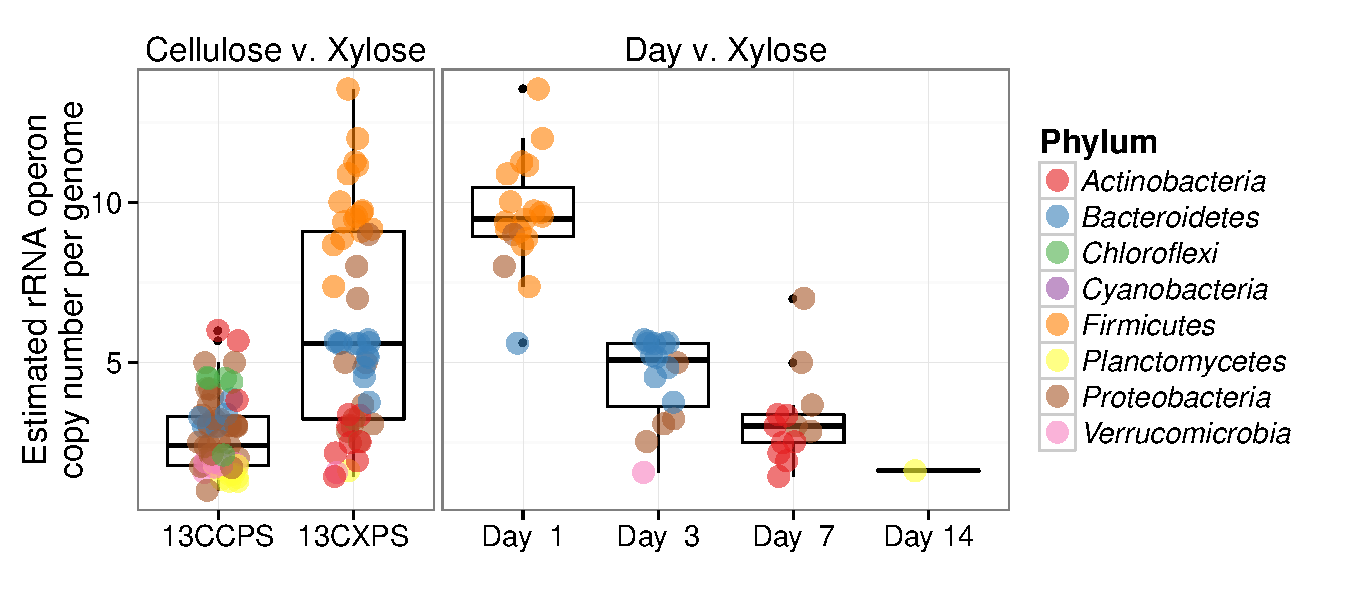
\includegraphics[width=\textwidth]{figures/copy_number/copy_number.pdf}}
	\caption{\protectEstimated rRNA operon copy number for xylose and cellulose responders. The
leftmost panel contrasts estimated \textit{rrn} copy number for cellulose (13CCPS) and 
xylose (13CXPS) responders. The right panel shows estimated \textit{rrn} copy number
versus time of first response for xylose responders. Colors denote the phylum
of the OTUs (see legend).

}\label{fig:copy}
        \end{center}
\end{figure*}

\begin{figure*}[H] \begin{center}
\centerline{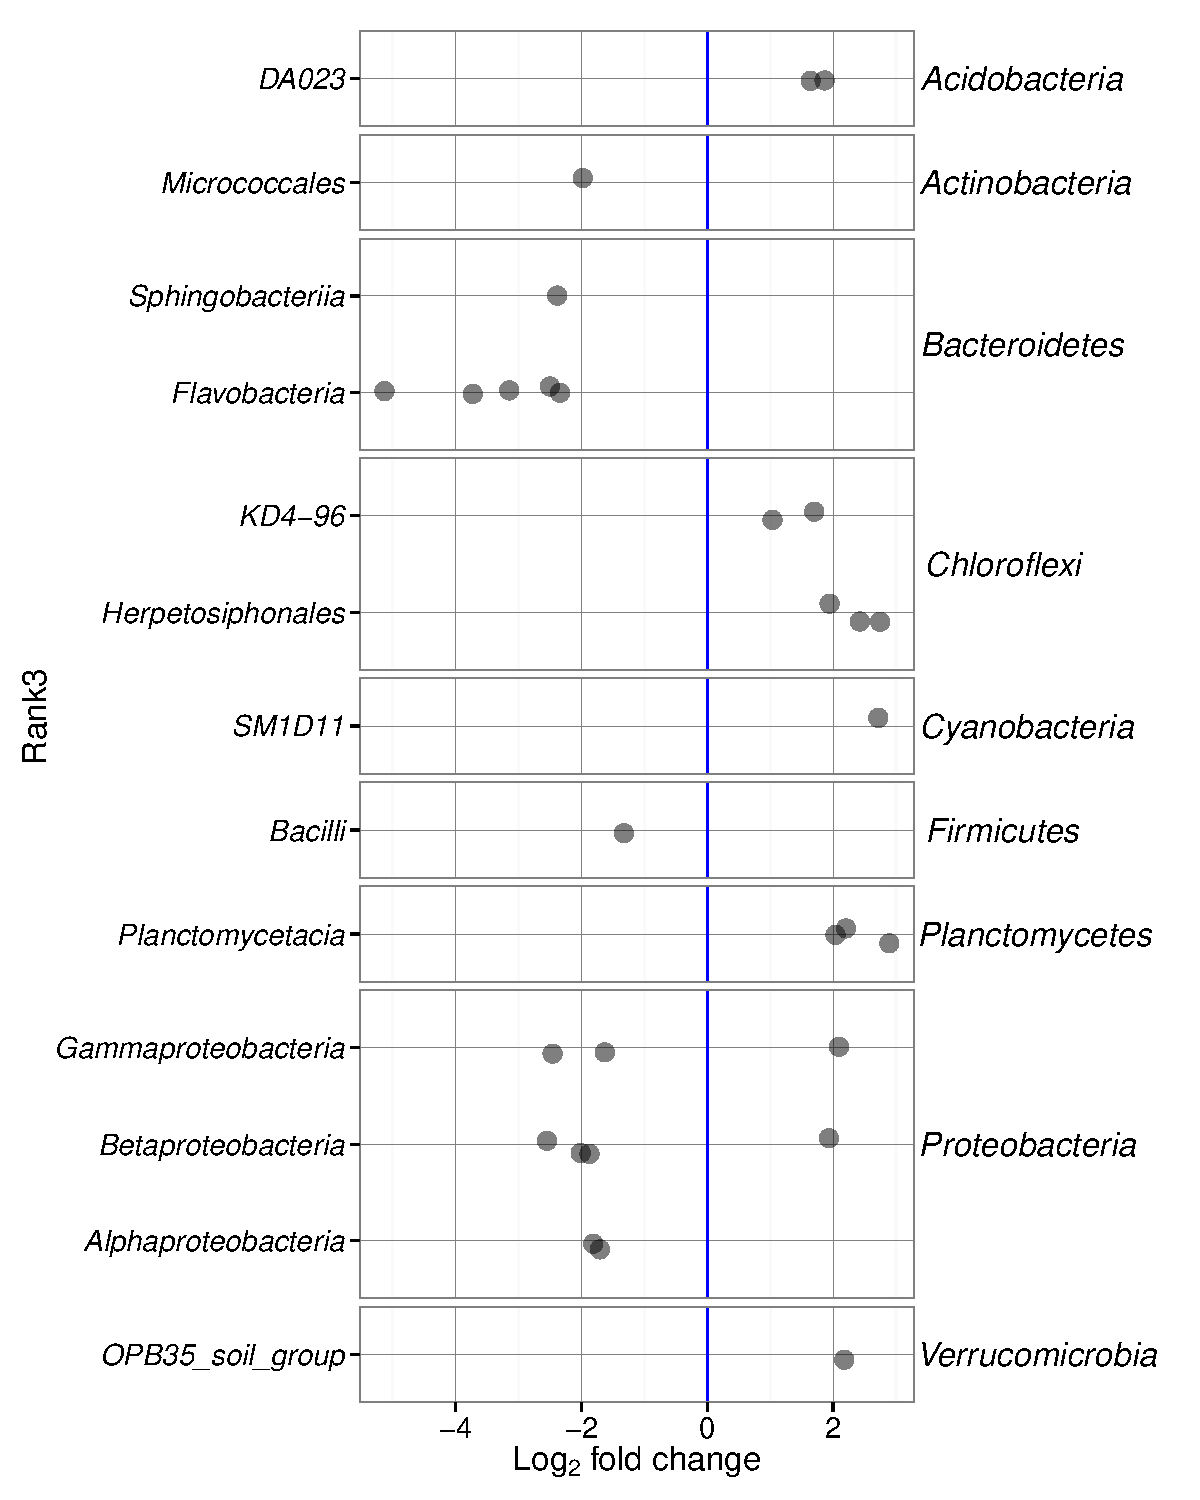
\includegraphics[width=0.75\textwidth]{figures/l2fc_time/l2fc_time.pdf}}
\caption{\protectFold change time$^{-1}$ for OTUs that changed significantly in abundance over time. One panel per phylum (phyla indicated on the right). Taxonomic class indicated on the left.}\label{fig:time}
\end{center} \end{figure*}

\begin{figure*}[H] \begin{center}
\centerline{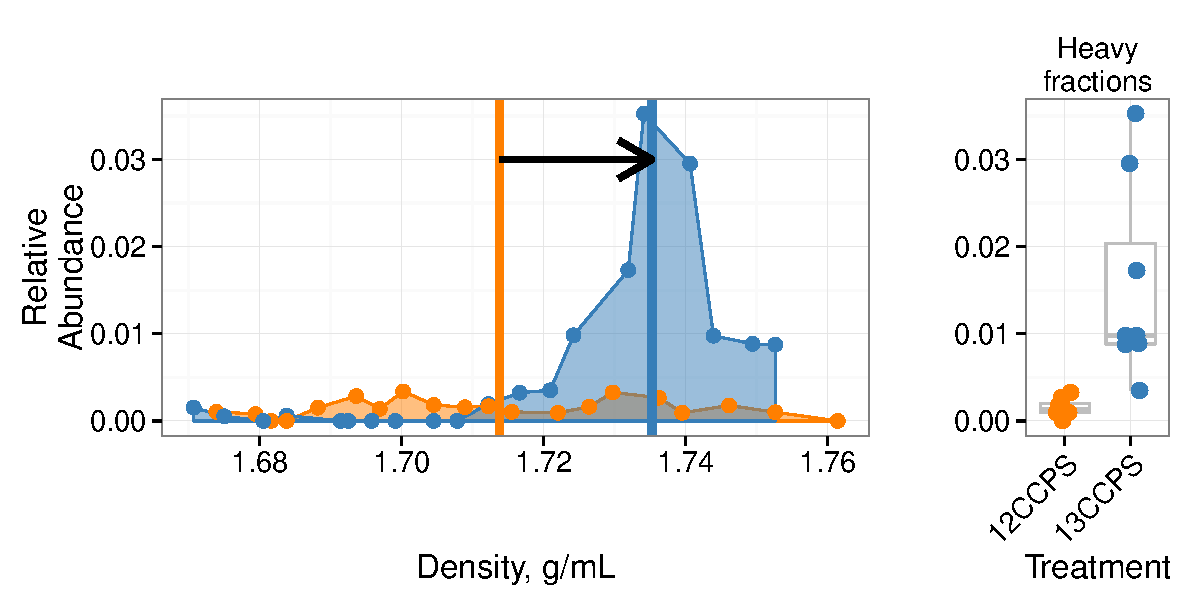
\includegraphics[width=0.75\textwidth]{figures/conceptual1/conceptual1.pdf}}
\caption{\protectDensity profile for a single $^13$C-cellulose "responder" OTU in the labeled gradient, blue, and the control gradient, orange. Vertical lines show center of mass for each density profile and arrow denotes the magnitude and direction of the BD shift upon labeling. Panel at right shows relative abundance values in the heavy fractions for each gradient. }\label{fig:c1}
\end{center} \end{figure*}

\begin{figure*}[H] \begin{center}
\centerline{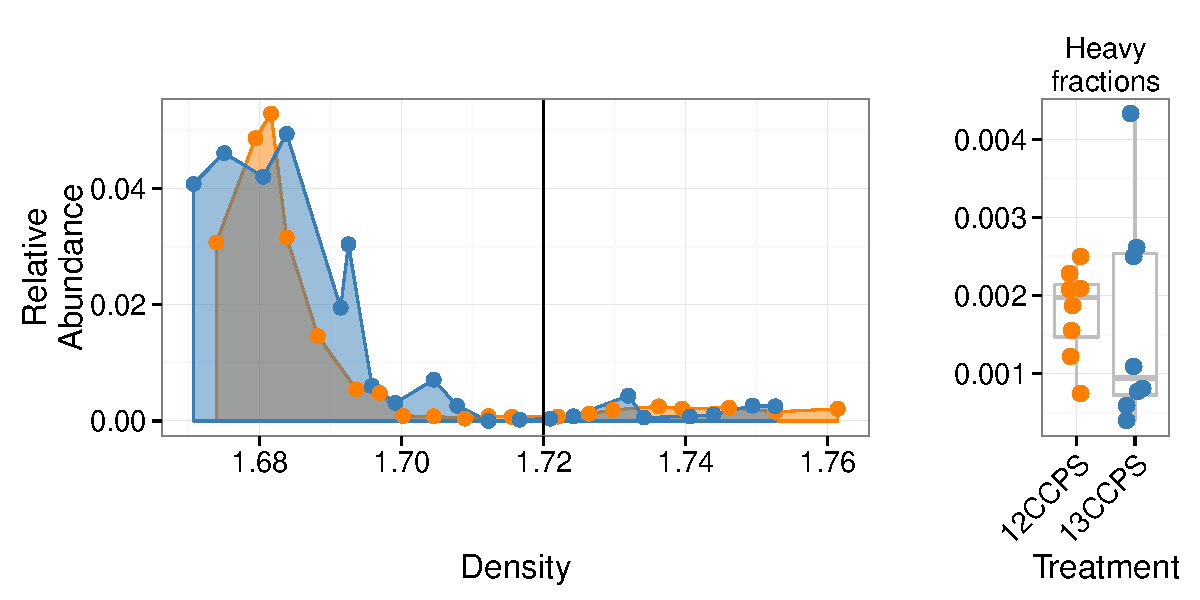
\includegraphics[width=0.75\textwidth]{figures/conceptual3/conceptual3.pdf}}
\caption{\protectDensity profile for a single non-responder OTU. The $^{13}$C-cellulose
treatment is in blue and the control treatment is in orange. The vertical line
shows where high density fractions begin as defined in our analysis. The right
panel shows relative abundance values in the high density fractions for each
gradient (The boxplot line is the median value. The box spans one
interquartile range (IR) about the median, whiskers extend 1.5 times the IR.  

}\label{fig:c3}
\end{center} \end{figure*}

\begin{figure*}[H]
	\begin{center}
    \centerline{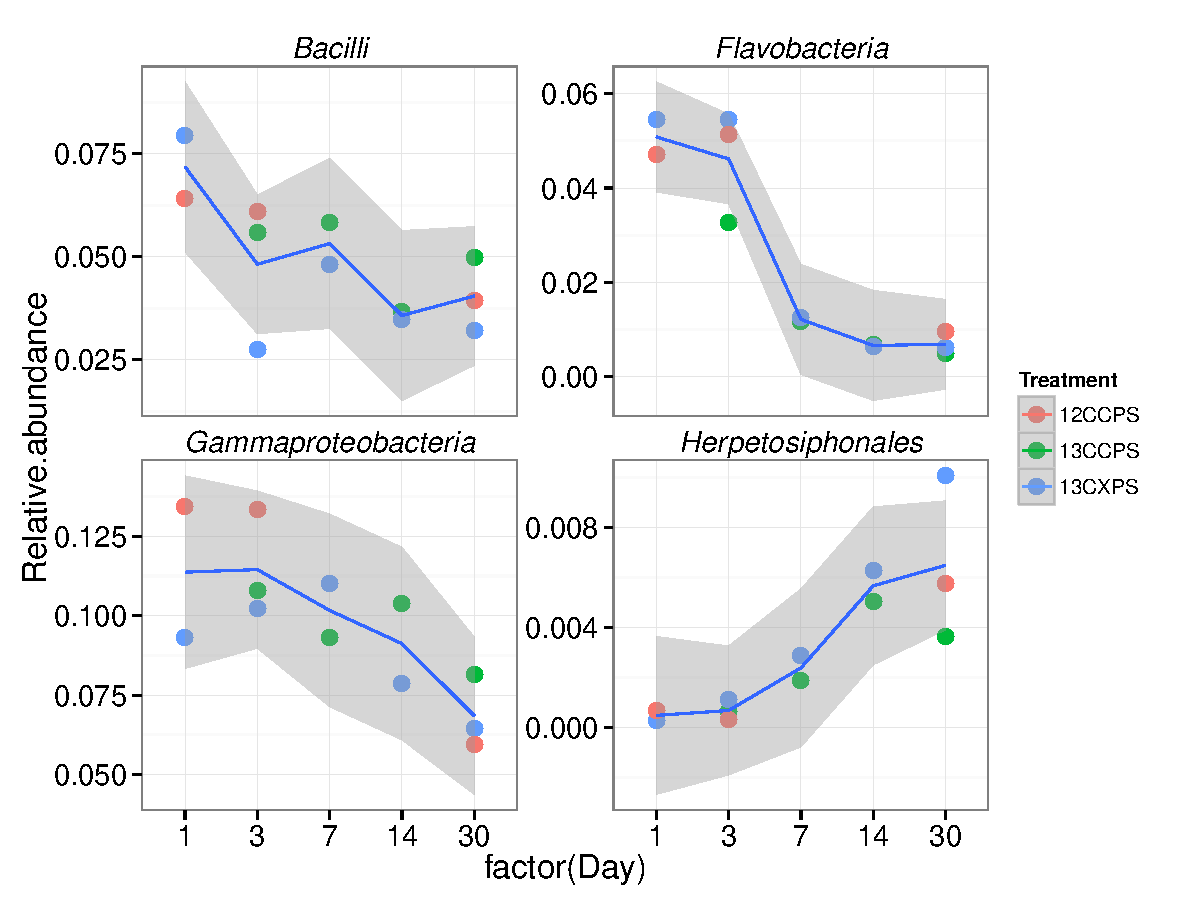
\includegraphics[width=0.85\textwidth]{figures/abndVtime_class/abndVtime_class.pdf}}
	\caption{\protectRelative abundance versus day for classes that changed significantly in relative abundance with time.}\label{fig:time_class}
    \end{center}
\end{figure*}

\begin{figure*}[H]
	\begin{center}
	\centerline{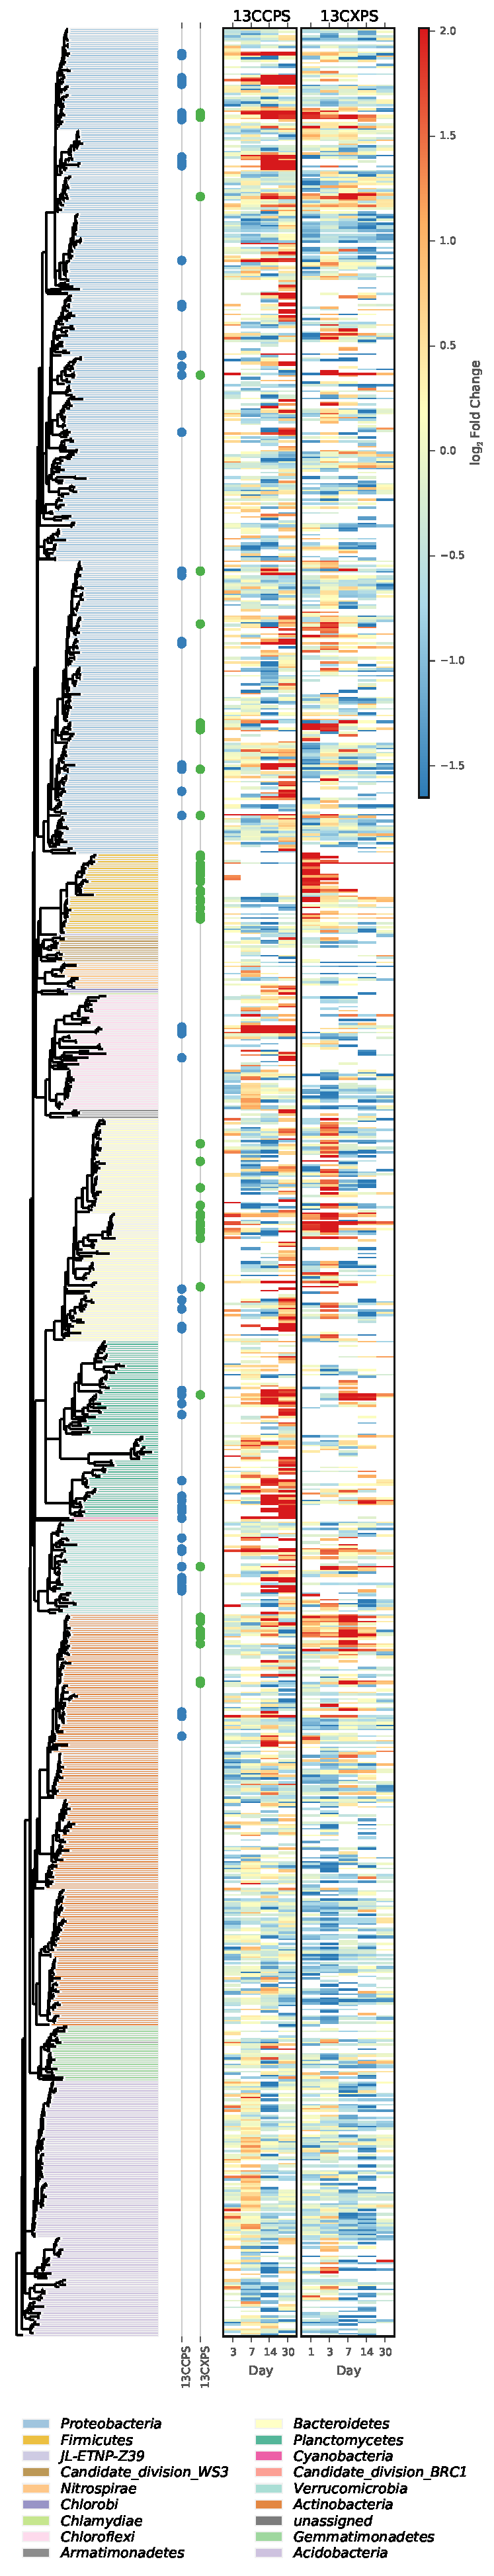
\includegraphics[width=0.25\textwidth]{figures/bacteria_tree/bacteria_tree.pdf}}
	\caption{\protectFigure 4. }\label{fig:trees}
        \end{center}
\end{figure*}

\begin{figure*}[H]
	\begin{center}
		\centerline{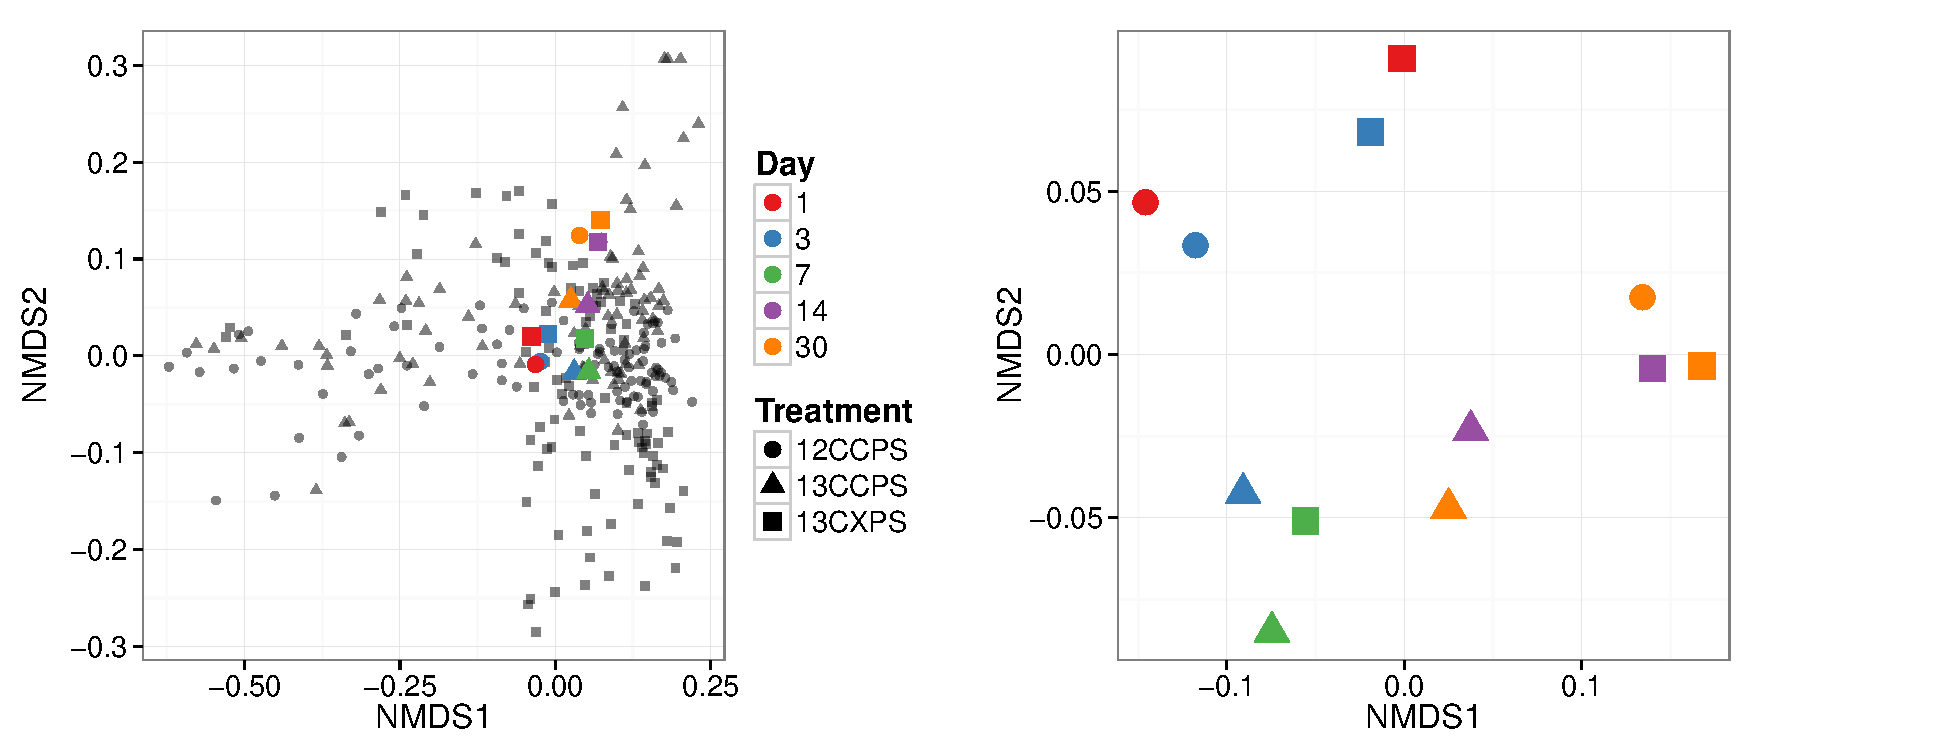
\includegraphics[width=\textwidth]{figures/bulk_ordination/bulk_ordination.pdf}}
	\caption{\protectNMDS analysis of SSU rRNA gene composition in non-fractionated DNA (colored points) indicates
that isotopic labelling does not alter overall microbial community composition,
microbial community composition in the soil microcosms changes over time, and
variance in non-fractionated DNA is smaller than variance in fractionated DNA (black points).
SSU rRNA gene sequences were determined for non-fractionated DNA from the
unlabeled control, $^{13}$C-xylose, and $^{13}$C-cellulose treatments over time (colors
indicate time, different symbols used for different treatments). Distance in SSU
rRNA gene composition was quantified with the UniFrac metric. The
leftmost panel indicates NMDS of data from both non-fractionated and
fractionated samples. The rightmost panel indicates NMDS of data only from
non-fractionated DNA. Statistical analysis is presented in main text.
}\label{fig:bulk_ord}
        \end{center}
\end{figure*}

\begin{figure*}[H]
	\begin{center}
    \centerline{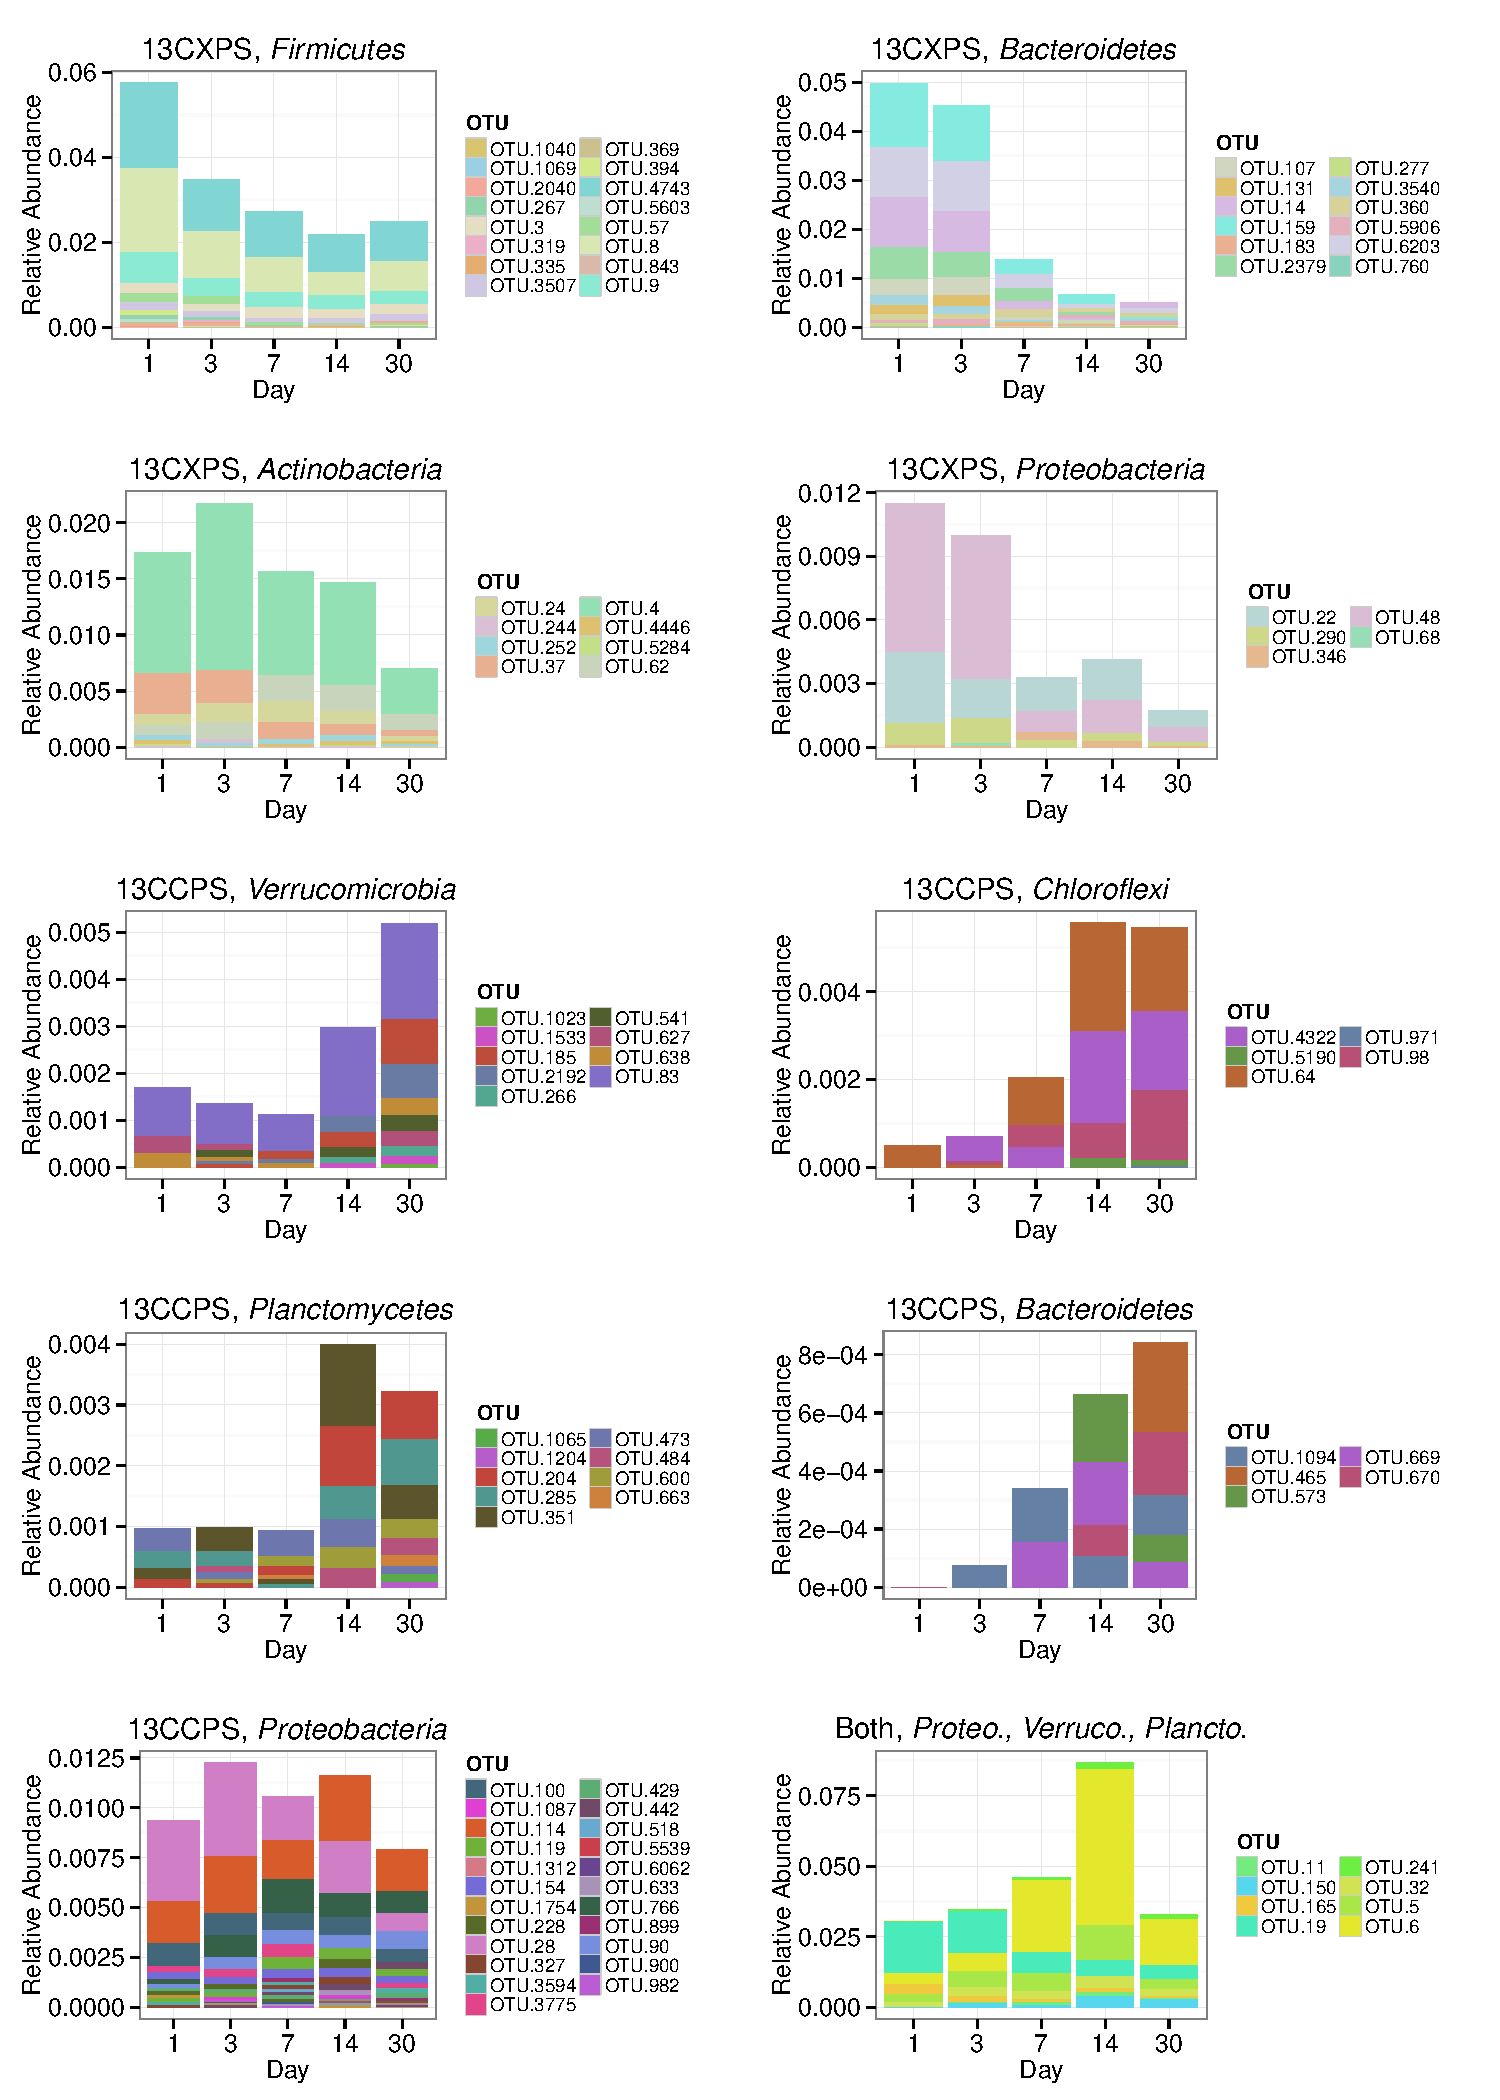
\includegraphics[width=0.75\textwidth]{figures/bulk_phylum_rspndr_abund/abund_v_time_phyla.pdf}}
	\caption{\protectChange in relative abundance in non-fractionated DNA over time for xylose
responders (13CXPS) and cellulose responders (13CCPS). Each panel represents
a phylum except for the lower right panel which shows all reponders to both
xylose and celluose. The abbreviations Proteo., Verruco., and Plancto.,
correspond to \textit{Proteobacteria}, \textit{Verrucomicrobia}, and \textit{Planctomycetes},
respectively.

}\label{fig:babund}
        \end{center}
\end{figure*}

\begin{figure*}[H]
	\begin{center}
	\centerline{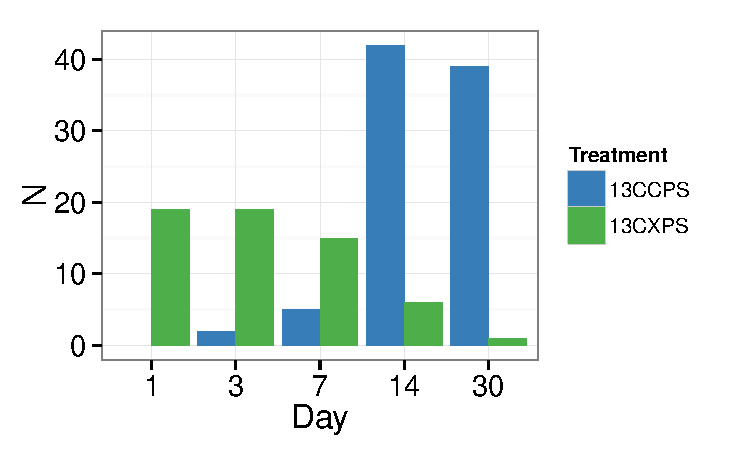
\includegraphics[width=0.75\textwidth]{figures/all_rspndr_bar/all_rspndr_bar.pdf}}
	\caption{\protectCounts of responders to each isotopically labeled substrate (cellulose and xylose) over time.}\label{fig:rspndr_count}
        \end{center}
\end{figure*}

\begin{figure*}[H]
	\begin{center}
    \centerline{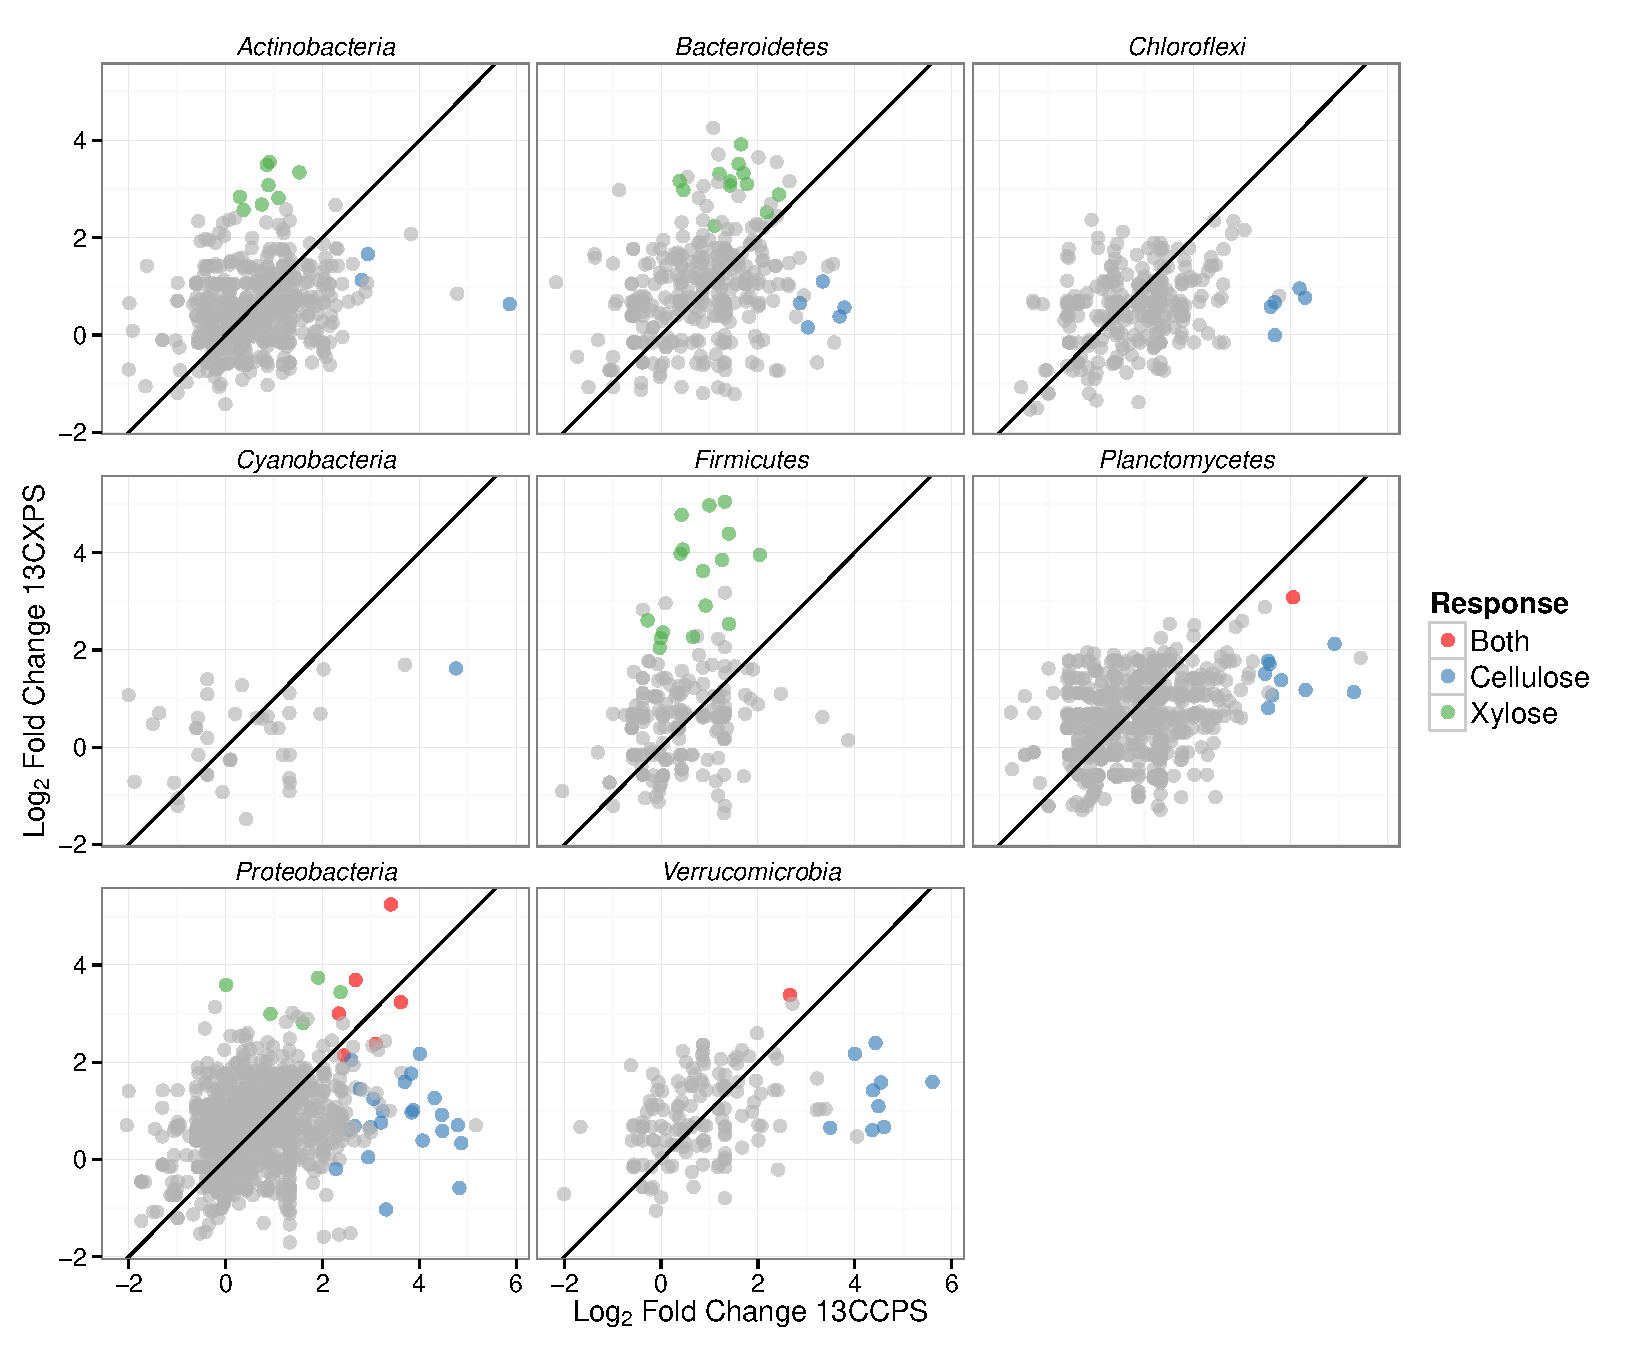
\includegraphics[width=\textwidth]{figures/generalist_specialist/generalist_specialist.pdf}}
    \caption{\protectMaximum enrichment at any point in time in heavy fractions of
$^{13}$C-treatments relative to controal (expressed as LFC) shown for
$^{13}$C-cellulose versus $^{13}$C-xylose treatments. Each point represents an
OTU. Blue points are cellulose responders, green xylose responders, and red are
responders to both xylose and cellulose, Grey points are OTUs that did not
repspond to either substrate. Line indicates a slope of one.
}\label{fig:genspec}
    \end{center} 
\end{figure*}

\begin{figure*}[H]
	\begin{center}
    \centerline{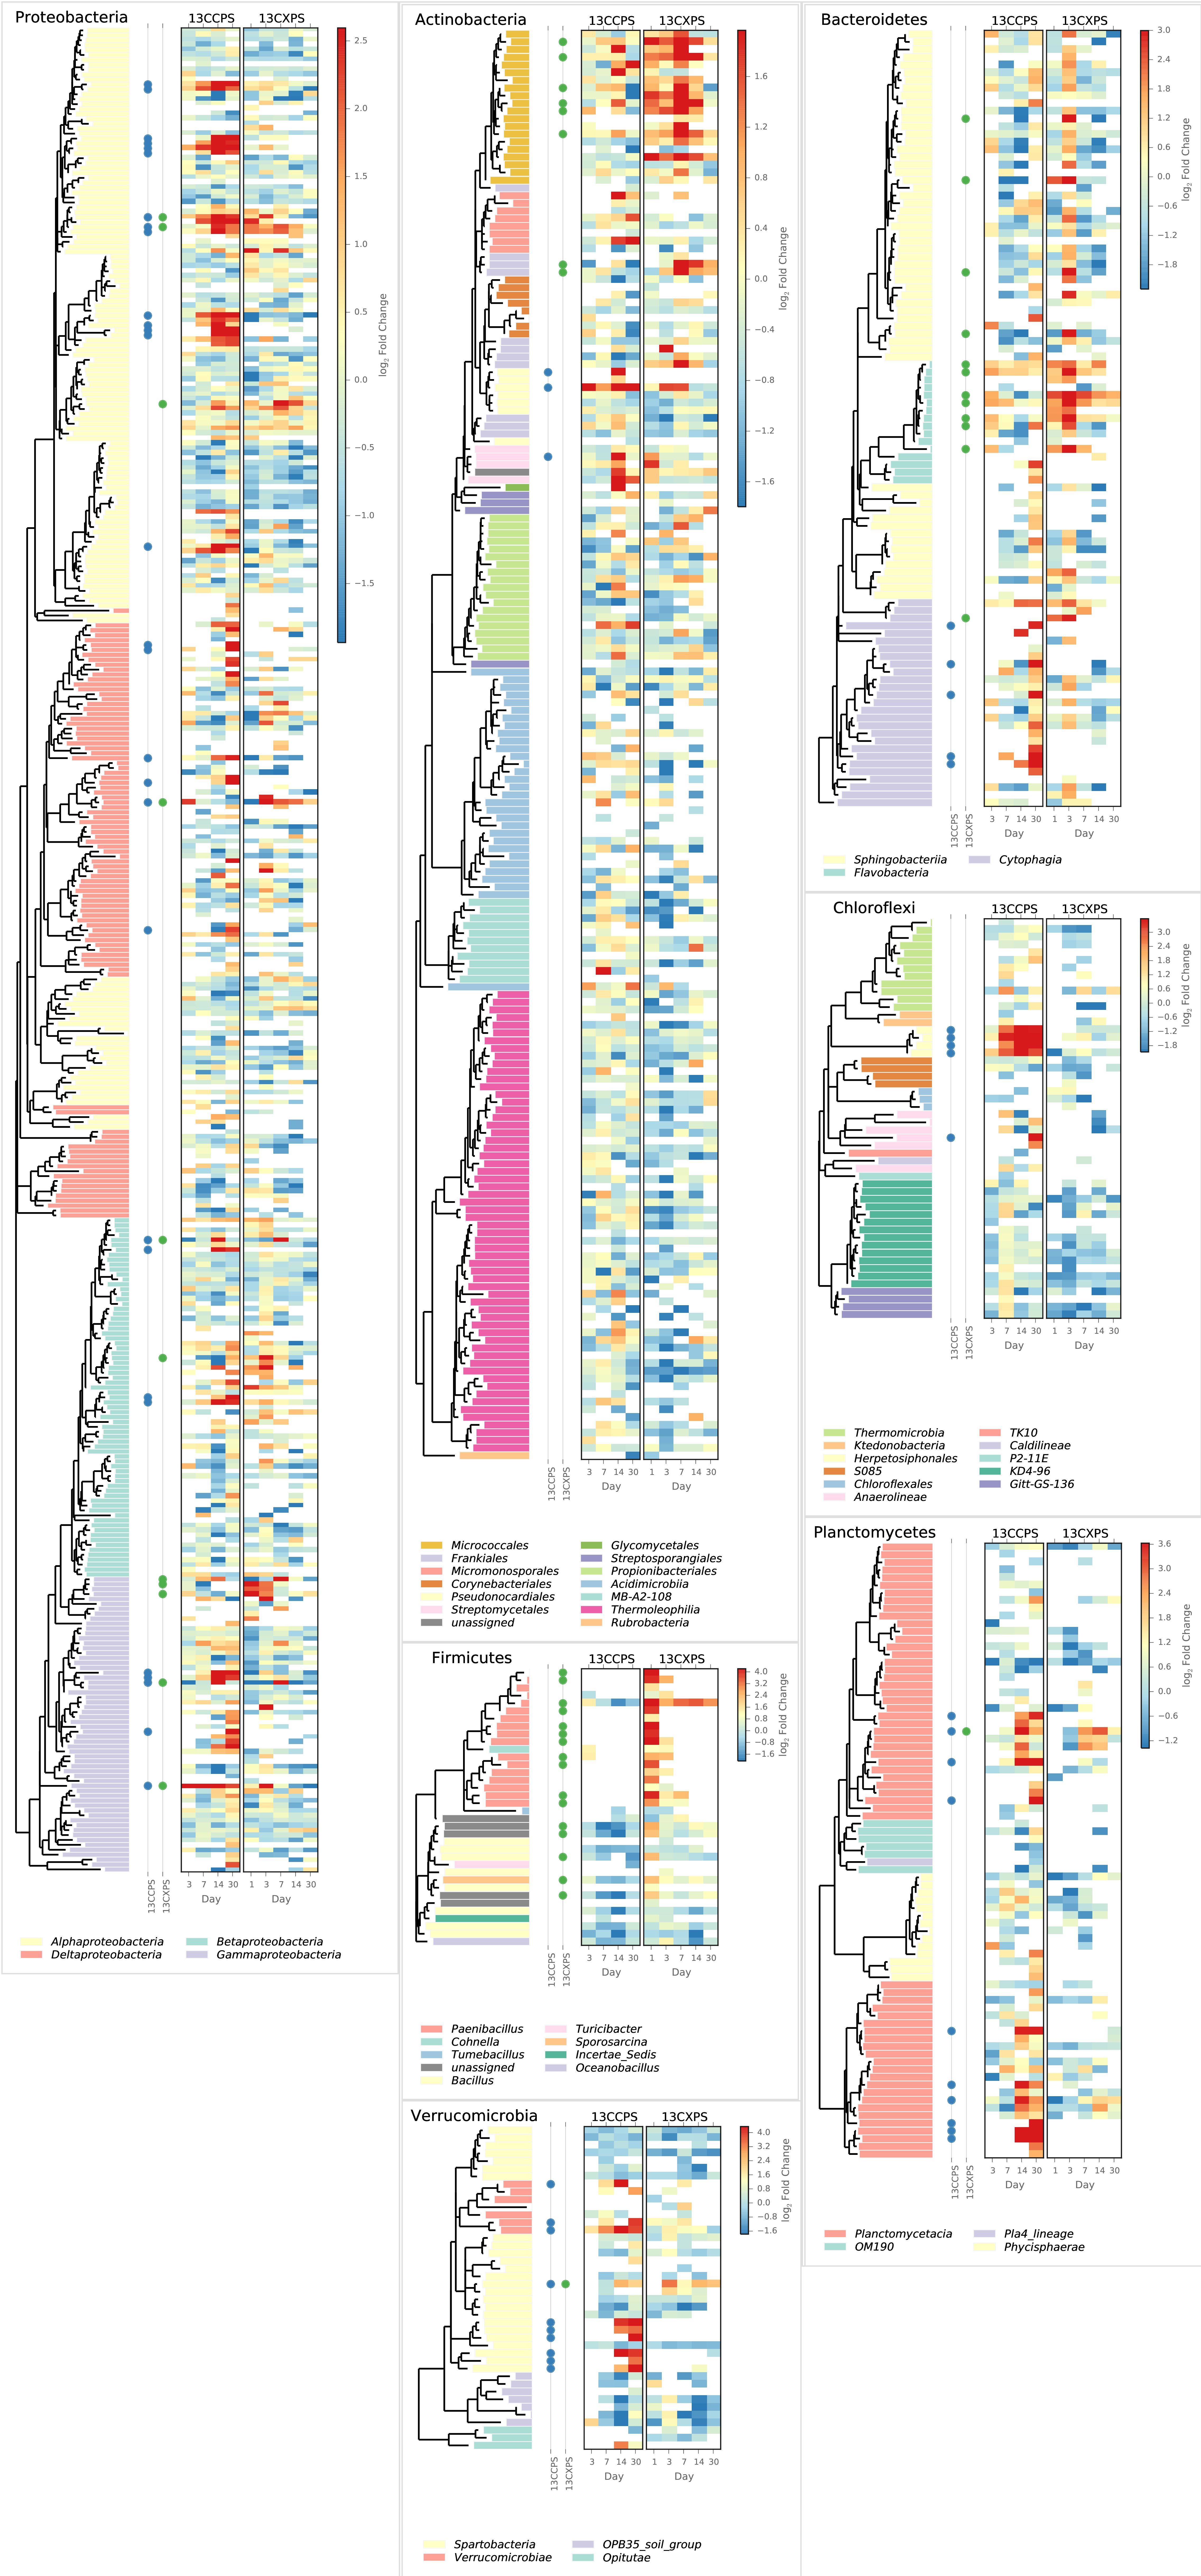
\includegraphics[width=0.65\textwidth]{figures/tiled_tree/tiled_tree.png}}
    \caption{\protectPhylogenetic position of cellulose responders and xylose responders in the context of all OTUs that passed 
sparsity independent filtering criteria (see Methods). Only those phyla that contain responders are shown.
Colored dots are used to identify xylose responders (green) and cellulse
responders (blue). The heatmaps indicate enrichment in high denstiy fractions
relative to control (represented as LFC) for each OTU in response to both
$^{13}$C-cellulose (13CCPS, leftmost heatmap) and $^{13}$C-xylose
(13CXPS, rightmost heatmap) with values for different days in each heatmap
column. High enrichment values (represented as LFC) provide evidence of $^{13}$C-labeled DNA.  

}\label{fig:tiledtree}
    \end{center} 
\end{figure*}

\begin{figure*}[H]
	\begin{center}
    \centerline{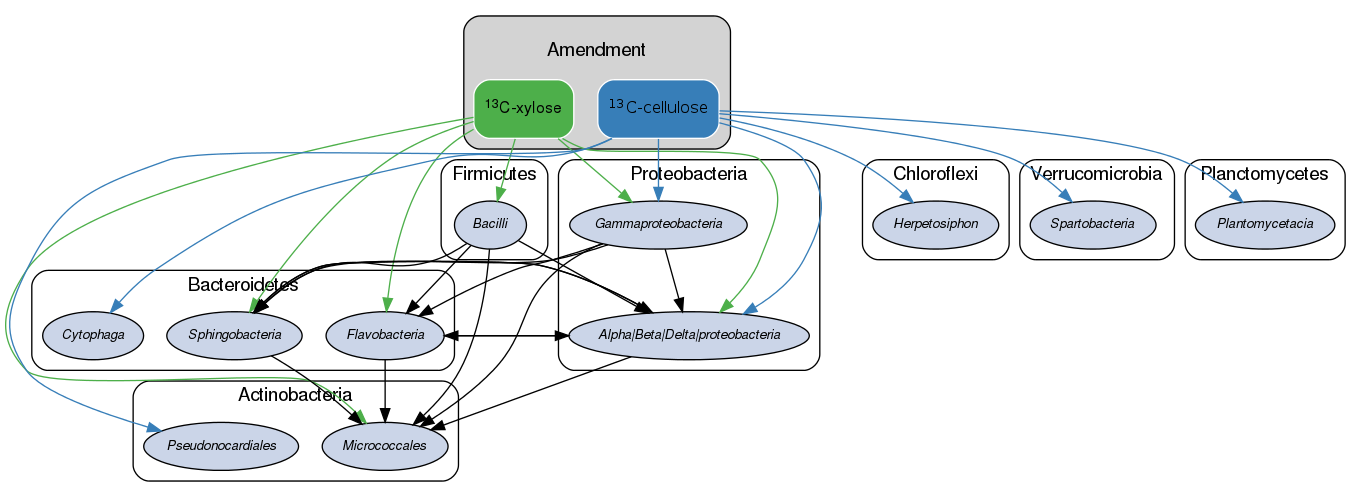
\includegraphics[width=0.75\textwidth]{figures/foodweb/foodweb.png}}
    \caption{\protectConceptual model of soil food web in this experiment.}\label{fig:foodweb}
    \end{center} 
\end{figure*}

\begin{longtable}{lrp{5cm}rp{7cm}}

\caption{$^{13}$C-cellulose responders BLAST against Living Tree Project} \\
\toprule \\
    \textbf{OTU ID} & \textbf{Fold change} & \textbf{Top BLAST hits} & \textbf{BLAST \%ID} & \textbf{Phylum;Class;Order} \\
\midrule
\endfirsthead

\multicolumn{3}{c}
{{\tablename\ \thetable{} -- continued from previous page}} \\
\midrule
    \textbf{OTU ID} & \textbf{Fold change} & \textbf{Top BLAST hits} & \textbf{BLAST \%ID} & \textbf{Phylum;Class;Order} \\
\midrule
\endhead
    OTU.862 & 5.87 & \mbox{\textit{Allokutzneria albata}} & 100.0 & \mbox{\textit{Actinobacteria}} \mbox{\textit{Pseudonocardiales}} \mbox{\textit{Pseudonocardiaceae}} \\ \midrule
OTU.257 & 2.94 & \mbox{\textit{Lentzea waywayandensis}}, \mbox{\textit{Lentzea flaviverrucosa}} & 100.0 & \mbox{\textit{Actinobacteria}} \mbox{\textit{Pseudonocardiales}} \mbox{\textit{Pseudonocardiaceae}} \\ \midrule
OTU.132 & 2.81 & \mbox{\textit{Streptomyces spp.}} & 100.0 & \mbox{\textit{Actinobacteria}} \mbox{\textit{Streptomycetales}} \mbox{\textit{Streptomycetaceae}} \\ \midrule
OTU.465 & 3.79 & \mbox{\textit{Ohtaekwangia kribbensis}} & 92.73 & \mbox{\textit{Bacteroidetes}} \mbox{\textit{Cytophagia}} \mbox{\textit{Cytophagales}} \\ \midrule
OTU.1094 & 3.69 & \mbox{\textit{Sporocytophaga myxococcoides}} & 99.55 & \mbox{\textit{Bacteroidetes}} \mbox{\textit{Cytophagia}} \mbox{\textit{Cytophagales}} \\ \midrule
OTU.669 & 3.34 & \mbox{\textit{Ohtaekwangia koreensis}} & 92.69 & \mbox{\textit{Bacteroidetes}} \mbox{\textit{Cytophagia}} \mbox{\textit{Cytophagales}} \\ \midrule
OTU.573 & 3.03 & \mbox{\textit{Adhaeribacter aerophilus}} & 92.76 & \mbox{\textit{Bacteroidetes}} \mbox{\textit{Cytophagia}} \mbox{\textit{Cytophagales}} \\ \midrule
OTU.670 & 2.87 & \mbox{\textit{Adhaeribacter aerophilus}} & 91.78 & \mbox{\textit{Bacteroidetes}} \mbox{\textit{Cytophagia}} \mbox{\textit{Cytophagales}} \\ \midrule
OTU.971 & 3.68 & {No hits of at least 90\% identity} & 78.57 & \mbox{\textit{Chloroflexi}} \mbox{\textit{Anaerolineae}} \mbox{\textit{Anaerolineales}} \\ \midrule
OTU.64 & 4.31 & {No hits of at least 90\% identity} & 89.5 & \mbox{\textit{Chloroflexi}} \mbox{\textit{Herpetosiphonales}} \mbox{\textit{Herpetosiphonaceae}} \\ \midrule
OTU.4322 & 4.19 & {No hits of at least 90\% identity} & 89.14 & \mbox{\textit{Chloroflexi}} \mbox{\textit{Herpetosiphonales}} \mbox{\textit{Herpetosiphonaceae}} \\ \midrule
OTU.98 & 3.68 & {No hits of at least 90\% identity} & 88.18 & \mbox{\textit{Chloroflexi}} \mbox{\textit{Herpetosiphonales}} \mbox{\textit{Herpetosiphonaceae}} \\ \midrule
OTU.5190 & 3.6 & {No hits of at least 90\% identity} & 88.13 & \mbox{\textit{Chloroflexi}} \mbox{\textit{Herpetosiphonales}} \mbox{\textit{Herpetosiphonaceae}} \\ \midrule
OTU.120 & 4.76 & \mbox{\textit{Vampirovibrio chlorellavorus}} & 94.52 & \mbox{\textit{Cyanobacteria}} \mbox{\textit{SM1D11}} \mbox{\textit{uncultured-bacterium}} \\ \midrule
OTU.1065 & 5.31 & {No hits of at least 90\% identity} & 84.55 & \mbox{\textit{Planctomycetes}} \mbox{\textit{Planctomycetacia}} \mbox{\textit{Planctomycetales}} \\ \midrule
OTU.484 & 4.92 & {No hits of at least 90\% identity} & 89.09 & \mbox{\textit{Planctomycetes}} \mbox{\textit{Planctomycetacia}} \mbox{\textit{Planctomycetales}} \\ \midrule
OTU.1204 & 4.32 & \mbox{\textit{Planctomyces limnophilus}} & 91.78 & \mbox{\textit{Planctomycetes}} \mbox{\textit{Planctomycetacia}} \mbox{\textit{Planctomycetales}} \\ \midrule
OTU.150 & 4.06 & {No hits of at least 90\% identity} & 86.76 & \mbox{\textit{Planctomycetes}} \mbox{\textit{Planctomycetacia}} \mbox{\textit{Planctomycetales}} \\ \midrule
OTU.663 & 3.63 & \mbox{\textit{Pirellula staleyi DSM 6068}} & 90.87 & \mbox{\textit{Planctomycetes}} \mbox{\textit{Planctomycetacia}} \mbox{\textit{Planctomycetales}} \\ \midrule
OTU.473 & 3.58 & \mbox{\textit{Pirellula staleyi DSM 6068}} & 90.91 & \mbox{\textit{Planctomycetes}} \mbox{\textit{Planctomycetacia}} \mbox{\textit{Planctomycetales}} \\ \midrule
OTU.285 & 3.55 & \mbox{\textit{Blastopirellula marina}} & 90.87 & \mbox{\textit{Planctomycetes}} \mbox{\textit{Planctomycetacia}} \mbox{\textit{Planctomycetales}} \\ \midrule
OTU.351 & 3.54 & \mbox{\textit{Pirellula staleyi DSM 6068}} & 91.86 & \mbox{\textit{Planctomycetes}} \mbox{\textit{Planctomycetacia}} \mbox{\textit{Planctomycetales}} \\ \midrule
OTU.600 & 3.48 & {No hits of at least 90\% identity} & 80.37 & \mbox{\textit{Planctomycetes}} \mbox{\textit{Planctomycetacia}} \mbox{\textit{Planctomycetales}} \\ \midrule
OTU.900 & 4.87 & \mbox{\textit{Brevundimonas vesicularis}}, \mbox{\textit{Brevundimonas nasdae}} & 100.0 & \mbox{\textit{Proteobacteria}} \mbox{\textit{Alphaproteobacteria}} \mbox{\textit{Caulobacterales}} \\ \midrule
OTU.1754 & 4.48 & \mbox{\textit{Asticcacaulis biprosthecium}}, \mbox{\textit{Asticcacaulis benevestitus}} & 96.8 & \mbox{\textit{Proteobacteria}} \mbox{\textit{Alphaproteobacteria}} \mbox{\textit{Caulobacterales}} \\ \midrule
OTU.119 & 3.31 & \mbox{\textit{Brevundimonas alba}} & 100.0 & \mbox{\textit{Proteobacteria}} \mbox{\textit{Alphaproteobacteria}} \mbox{\textit{Caulobacterales}} \\ \midrule
OTU.327 & 2.99 & \mbox{\textit{Asticcacaulis biprosthecium}}, \mbox{\textit{Asticcacaulis benevestitus}} & 98.63 & \mbox{\textit{Proteobacteria}} \mbox{\textit{Alphaproteobacteria}} \mbox{\textit{Caulobacterales}} \\ \midrule
OTU.982 & 4.47 & \mbox{\textit{Devosia neptuniae}} & 100.0 & \mbox{\textit{Proteobacteria}} \mbox{\textit{Alphaproteobacteria}} \mbox{\textit{Rhizobiales}} \\ \midrule
OTU.1087 & 4.32 & \mbox{\textit{Devosia soli}}, \mbox{\textit{Devosia crocina}}, \mbox{\textit{Devosia riboflavina}} & 99.09 & \mbox{\textit{Proteobacteria}} \mbox{\textit{Alphaproteobacteria}} \mbox{\textit{Rhizobiales}} \\ \midrule
OTU.5539 & 4.01 & \mbox{\textit{Devosia subaequoris}} & 98.17 & \mbox{\textit{Proteobacteria}} \mbox{\textit{Alphaproteobacteria}} \mbox{\textit{Rhizobiales}} \\ \midrule
OTU.3775 & 3.88 & \mbox{\textit{Devosia glacialis}}, \mbox{\textit{Devosia chinhatensis}}, \mbox{\textit{Devosia geojensis}}, \mbox{\textit{Devosia yakushimensis}} & 98.63 & \mbox{\textit{Proteobacteria}} \mbox{\textit{Alphaproteobacteria}} \mbox{\textit{Rhizobiales}} \\ \midrule
OTU.429 & 3.7 & \mbox{\textit{Devosia limi}}, \mbox{\textit{Devosia psychrophila}} & 97.72 & \mbox{\textit{Proteobacteria}} \mbox{\textit{Alphaproteobacteria}} \mbox{\textit{Rhizobiales}} \\ \midrule
OTU.766 & 3.21 & \mbox{\textit{Devosia insulae}} & 99.54 & \mbox{\textit{Proteobacteria}} \mbox{\textit{Alphaproteobacteria}} \mbox{\textit{Rhizobiales}} \\ \midrule
OTU.165 & 3.1 & \mbox{\textit{Rhizobium spp.}} & 100.0 & \mbox{\textit{Proteobacteria}} \mbox{\textit{Alphaproteobacteria}} \mbox{\textit{Rhizobiales}} \\ \midrule
OTU.28 & 2.59 & \mbox{\textit{Rhizobium giardinii}}, \mbox{\textit{Rhizobium tubonense}}, \mbox{\textit{Rhizobium tibeticum}}, \mbox{\textit{Rhizobium mesoamericanum CCGE 501}}, \mbox{\textit{Rhizobium herbae}}, \mbox{\textit{Rhizobium endophyticum}} & 99.54 & \mbox{\textit{Proteobacteria}} \mbox{\textit{Alphaproteobacteria}} \mbox{\textit{Rhizobiales}} \\ \midrule
OTU.19 & 2.44 & \mbox{\textit{Rhizobium spp.}}, \mbox{\textit{Arthrobacter spp.}} & 99.54 & \mbox{\textit{Proteobacteria}} \mbox{\textit{Alphaproteobacteria}} \mbox{\textit{Rhizobiales}} \\ \midrule
OTU.90 & 2.94 & \mbox{\textit{Sphingopyxis panaciterrae}}, \mbox{\textit{Sphingopyxis chilensis}}, \mbox{\textit{Sphingopyxis sp. BZ30}}, \mbox{\textit{Sphingomonas sp.}} & 100.0 & \mbox{\textit{Proteobacteria}} \mbox{\textit{Alphaproteobacteria}} \mbox{\textit{Sphingomonadales}} \\ \midrule
OTU.518 & 4.8 & \mbox{\textit{Hydrogenophaga intermedia}} & 100.0 & \mbox{\textit{Proteobacteria}} \mbox{\textit{Betaproteobacteria}} \mbox{\textit{Burkholderiales}} \\ \midrule
OTU.1312 & 4.07 & \mbox{\textit{Paucimonas lemoignei}} & 99.54 & \mbox{\textit{Proteobacteria}} \mbox{\textit{Betaproteobacteria}} \mbox{\textit{Burkholderiales}} \\ \midrule
OTU.5 & 3.69 & \mbox{\textit{Delftia tsuruhatensis}}, \mbox{\textit{Delftia lacustris}} & 100.0 & \mbox{\textit{Proteobacteria}} \mbox{\textit{Betaproteobacteria}} \mbox{\textit{Burkholderiales}} \\ \midrule
OTU.114 & 2.78 & \mbox{\textit{Herbaspirillum sp. SUEMI03}}, \mbox{\textit{Herbaspirillum sp. SUEMI10}}, \mbox{\textit{Oxalicibacterium solurbis}}, \mbox{\textit{Herminiimonas fonticola}}, \mbox{\textit{Oxalicibacterium horti}} & 100.0 & \mbox{\textit{Proteobacteria}} \mbox{\textit{Betaproteobacteria}} \mbox{\textit{Burkholderiales}} \\ \midrule
OTU.633 & 3.84 & {No hits of at least 90\% identity} & 89.5 & \mbox{\textit{Proteobacteria}} \mbox{\textit{Deltaproteobacteria}} \mbox{\textit{Myxococcales}} \\ \midrule
OTU.3594 & 3.83 & \mbox{\textit{Chondromyces robustus}} & 90.41 & \mbox{\textit{Proteobacteria}} \mbox{\textit{Deltaproteobacteria}} \mbox{\textit{Myxococcales}} \\ \midrule
OTU.442 & 3.05 & \mbox{\textit{Chondromyces robustus}} & 92.24 & \mbox{\textit{Proteobacteria}} \mbox{\textit{Deltaproteobacteria}} \mbox{\textit{Myxococcales}} \\ \midrule
OTU.32 & 3.0 & \mbox{\textit{Sandaracinus amylolyticus}} & 94.98 & \mbox{\textit{Proteobacteria}} \mbox{\textit{Deltaproteobacteria}} \mbox{\textit{Myxococcales}} \\ \midrule
OTU.228 & 2.54 & \mbox{\textit{Sorangium cellulosum}} & 98.17 & \mbox{\textit{Proteobacteria}} \mbox{\textit{Deltaproteobacteria}} \mbox{\textit{Myxococcales}} \\ \midrule
OTU.899 & 2.28 & \mbox{\textit{Enhygromyxa salina}} & 97.72 & \mbox{\textit{Proteobacteria}} \mbox{\textit{Deltaproteobacteria}} \mbox{\textit{Myxococcales}} \\ \midrule
OTU.6 & 3.62 & \mbox{\textit{Cellvibrio fulvus}} & 100.0 & \mbox{\textit{Proteobacteria}} \mbox{\textit{Gammaproteobacteria}} \mbox{\textit{Pseudomonadales}} \\ \midrule
OTU.11 & 5.25 & \mbox{\textit{Stenotrophomonas pavanii}}, \mbox{\textit{Stenotrophomonas maltophilia}}, \mbox{\textit{Pseudomonas geniculata}} & 99.54 & \mbox{\textit{Proteobacteria}} \mbox{\textit{Gammaproteobacteria}} \mbox{\textit{Xanthomonadales}} \\ \midrule
OTU.6062 & 4.83 & \mbox{\textit{Dokdonella sp. DC-3}}, \mbox{\textit{Luteibacter rhizovicinus}} & 97.26 & \mbox{\textit{Proteobacteria}} \mbox{\textit{Gammaproteobacteria}} \mbox{\textit{Xanthomonadales}} \\ \midrule
OTU.154 & 3.24 & \mbox{\textit{Pseudoxanthomonas mexicana}}, \mbox{\textit{Pseudoxanthomonas japonensis}} & 100.0 & \mbox{\textit{Proteobacteria}} \mbox{\textit{Gammaproteobacteria}} \mbox{\textit{Xanthomonadales}} \\ \midrule
OTU.100 & 2.66 & \mbox{\textit{Pseudoxanthomonas sacheonensis}}, \mbox{\textit{Pseudoxanthomonas dokdonensis}} & 100.0 & \mbox{\textit{Proteobacteria}} \mbox{\textit{Gammaproteobacteria}} \mbox{\textit{Xanthomonadales}} \\ \midrule
OTU.1023 & 4.61 & {No hits of at least 90\% identity} & 80.54 & \mbox{\textit{Verrucomicrobia}} \mbox{\textit{Spartobacteria}} \mbox{\textit{Chthoniobacterales}} \\ \midrule
OTU.266 & 4.54 & {No hits of at least 90\% identity} & 83.64 & \mbox{\textit{Verrucomicrobia}} \mbox{\textit{Spartobacteria}} \mbox{\textit{Chthoniobacterales}} \\ \midrule
OTU.541 & 4.49 & {No hits of at least 90\% identity} & 84.23 & \mbox{\textit{Verrucomicrobia}} \mbox{\textit{Spartobacteria}} \mbox{\textit{Chthoniobacterales}} \\ \midrule
OTU.185 & 4.37 & {No hits of at least 90\% identity} & 85.14 & \mbox{\textit{Verrucomicrobia}} \mbox{\textit{Spartobacteria}} \mbox{\textit{Chthoniobacterales}} \\ \midrule
OTU.2192 & 3.49 & {No hits of at least 90\% identity} & 83.56 & \mbox{\textit{Verrucomicrobia}} \mbox{\textit{Spartobacteria}} \mbox{\textit{Chthoniobacterales}} \\ \midrule
OTU.1533 & 3.43 & {No hits of at least 90\% identity} & 82.27 & \mbox{\textit{Verrucomicrobia}} \mbox{\textit{Spartobacteria}} \mbox{\textit{Chthoniobacterales}} \\ \midrule
OTU.241 & 3.38 & {No hits of at least 90\% identity} & 87.73 & \mbox{\textit{Verrucomicrobia}} \mbox{\textit{Spartobacteria}} \mbox{\textit{Chthoniobacterales}} \\ \midrule
OTU.83 & 5.61 & \mbox{\textit{Luteolibacter sp. CCTCC AB 2010415}} & 97.72 & \mbox{\textit{Verrucomicrobia}} \mbox{\textit{Verrucomicrobiae}} \mbox{\textit{Verrucomicrobiales}} \\ \midrule
OTU.627 & 4.43 & \mbox{\textit{Verrucomicrobiaceae bacterium DC2a-G7}} & 100.0 & \mbox{\textit{Verrucomicrobia}} \mbox{\textit{Verrucomicrobiae}} \mbox{\textit{Verrucomicrobiales}} \\ \midrule
OTU.638 & 4.0 & \mbox{\textit{Luteolibacter sp. CCTCC AB 2010415}}, \mbox{\textit{Luteolibacter algae}} & 93.61 & \mbox{\textit{Verrucomicrobia}} \mbox{\textit{Verrucomicrobiae}} \mbox{\textit{Verrucomicrobiales}} \\ \midrule

\bottomrule
\label{tab:cell}
\end{longtable}

\thispagestyle{empty}
\newgeometry{tmargin=2cm, bmargin=2cm, lmargin=0.25cm, rmargin=0.25cm} 

\begin{ThreePartTable}
\begin{TableNotes}
\item[a] Maximum observed $log_{2}$ of fold change. 
\item[b] Day of maximum fold change.
\item[c] All response days.
\end{TableNotes}

\begin{longtable}{P{1.5cm}rP{1cm}P{1.5cm}P{4cm}rP{5cm}}

\caption{$^{13}$C-xylose responders BLAST against Living Tree Project} \\
\label{tab:xyl}
\toprule 
    \textbf{OTU ID} & 
    \textbf{Fold change} \tnote{a} & 
    \textbf{Day} \tnote{b} & 
    \textbf{All days} \tnote{c} &
    \textbf{Top BLAST hits} & 
    \textbf{BLAST \%ID} & 
    \textbf{Phylum;Class;Order} \\
\midrule
\endfirsthead

\multicolumn{3}{c}
{{\tablename\ \thetable{} -- continued from previous page}} \\
\midrule
    \textbf{OTU ID} & 
    \textbf{Fold change} & 
    \textbf{Day} & 
    \textbf{All days} &
    \textbf{Top BLAST hits} & 
    \textbf{BLAST \%ID} & 
    \textbf{Phylum;Class;Order} \\
\midrule
\endhead
    OTU.1040 & 4.78 & 1 & 1&\mbox{\textit{Paenibacillus daejeonensis}} & 100.0 & \mbox{\textit{Firmicutes}} \mbox{\textit{Bacilli}} \mbox{\textit{Bacillales}} \\ \midrule
OTU.1069 & 3.85 & 1 & 1&\mbox{\textit{Paenibacillus terrigena}} & 100.0 & \mbox{\textit{Firmicutes}} \mbox{\textit{Bacilli}} \mbox{\textit{Bacillales}} \\ \midrule
OTU.107 & 2.25 & 3 & 3&\mbox{\textit{Flavobacterium sp. 15C3}}, \mbox{\textit{Flavobacterium banpakuense}} & 99.54 & \mbox{\textit{Bacteroidetes}} \mbox{\textit{Flavobacteria}} \mbox{\textit{Flavobacteriales}} \\ \midrule
OTU.11 & 5.25 & 7 & 7&\mbox{\textit{Stenotrophomonas pavanii}}, \mbox{\textit{Stenotrophomonas maltophilia}}, \mbox{\textit{Pseudomonas geniculata}} & 99.54 & \mbox{\textit{Proteobacteria}} \mbox{\textit{Gammaproteobacteria}} \mbox{\textit{Xanthomonadales}} \\ \midrule
OTU.131 & 3.07 & 3 & 3&\mbox{\textit{Flavobacterium fluvii}}, \mbox{\textit{Flavobacteria bacterium HMD1033}}, \mbox{\textit{Flavobacterium sp. HMD1001}} & 100.0 & \mbox{\textit{Bacteroidetes}} \mbox{\textit{Flavobacteria}} \mbox{\textit{Flavobacteriales}} \\ \midrule
OTU.14 & 3.92 & 3 & 1, 3&\mbox{\textit{Flavobacterium oncorhynchi}}, \mbox{\textit{Flavobacterium glycines}}, \mbox{\textit{Flavobacterium succinicans}} & 99.09 & \mbox{\textit{Bacteroidetes}} \mbox{\textit{Flavobacteria}} \mbox{\textit{Flavobacteriales}} \\ \midrule
OTU.150 & 3.08 & 14 & 14&{No hits of at least 90\% identity} & 86.76 & \mbox{\textit{Planctomycetes}} \mbox{\textit{Planctomycetacia}} \mbox{\textit{Planctomycetales}} \\ \midrule
OTU.159 & 3.16 & 3 & 3&\mbox{\textit{Flavobacterium hibernum}} & 98.17 & \mbox{\textit{Bacteroidetes}} \mbox{\textit{Flavobacteria}} \mbox{\textit{Flavobacteriales}} \\ \midrule
OTU.165 & 2.38 & 3 & 3&\mbox{\textit{Rhizobium skierniewicense}}, \mbox{\textit{Rhizobium vignae}}, \mbox{\textit{Rhizobium larrymoorei}}, \mbox{\textit{Rhizobium alkalisoli}}, \mbox{\textit{Rhizobium galegae}}, \mbox{\textit{Rhizobium huautlense}} & 100.0 & \mbox{\textit{Proteobacteria}} \mbox{\textit{Alphaproteobacteria}} \mbox{\textit{Rhizobiales}} \\ \midrule
OTU.183 & 3.31 & 3 & 3&{No hits of at least 90\% identity} & 89.5 & \mbox{\textit{Bacteroidetes}} \mbox{\textit{Sphingobacteriia}} \mbox{\textit{Sphingobacteriales}} \\ \midrule
OTU.19 & 2.14 & 7 & 7&\mbox{\textit{Rhizobium alamii}}, \mbox{\textit{Rhizobium mesosinicum}}, \mbox{\textit{Rhizobium mongolense}}, \mbox{\textit{Arthrobacter viscosus}}, \mbox{\textit{Rhizobium sullae}}, \mbox{\textit{Rhizobium yanglingense}}, \mbox{\textit{Rhizobium loessense}} & 99.54 & \mbox{\textit{Proteobacteria}} \mbox{\textit{Alphaproteobacteria}} \mbox{\textit{Rhizobiales}} \\ \midrule
OTU.2040 & 2.91 & 1 & 1&\mbox{\textit{Paenibacillus pectinilyticus}} & 100.0 & \mbox{\textit{Firmicutes}} \mbox{\textit{Bacilli}} \mbox{\textit{Bacillales}} \\ \midrule
OTU.22 & 2.8 & 7 & 7, 14&\mbox{\textit{Paracoccus sp. NB88}} & 99.09 & \mbox{\textit{Proteobacteria}} \mbox{\textit{Alphaproteobacteria}} \mbox{\textit{Rhodobacterales}} \\ \midrule
OTU.2379 & 3.1 & 3 & 3&\mbox{\textit{Flavobacterium pectinovorum}}, \mbox{\textit{Flavobacterium sp. CS100}} & 97.72 & \mbox{\textit{Bacteroidetes}} \mbox{\textit{Flavobacteria}} \mbox{\textit{Flavobacteriales}} \\ \midrule
OTU.24 & 2.81 & 7 & 7&\mbox{\textit{Cellulomonas aerilata}}, \mbox{\textit{Cellulomonas humilata}}, \mbox{\textit{Cellulomonas terrae}}, \mbox{\textit{Cellulomonas soli}}, \mbox{\textit{Cellulomonas xylanilytica}} & 100.0 & \mbox{\textit{Actinobacteria}} \mbox{\textit{Micrococcales}} \mbox{\textit{Cellulomonadaceae}} \\ \midrule
OTU.241 & 3.38 & 3 & 3, 14&{No hits of at least 90\% identity} & 87.73 & \mbox{\textit{Verrucomicrobia}} \mbox{\textit{Spartobacteria}} \mbox{\textit{Chthoniobacterales}} \\ \midrule
OTU.244 & 3.08 & 7 & 7&\mbox{\textit{Cellulosimicrobium funkei}}, \mbox{\textit{Cellulosimicrobium terreum}} & 100.0 & \mbox{\textit{Actinobacteria}} \mbox{\textit{Micrococcales}} \mbox{\textit{Promicromonosporaceae}} \\ \midrule
OTU.252 & 3.34 & 7 & 7&\mbox{\textit{Promicromonospora thailandica}} & 100.0 & \mbox{\textit{Actinobacteria}} \mbox{\textit{Micrococcales}} \mbox{\textit{Promicromonosporaceae}} \\ \midrule
OTU.267 & 4.97 & 1 & 1&\mbox{\textit{Paenibacillus pabuli}}, \mbox{\textit{Paenibacillus tundrae}}, \mbox{\textit{Paenibacillus taichungensis}}, \mbox{\textit{Paenibacillus xylanexedens}}, \mbox{\textit{Paenibacillus xylanilyticus}} & 100.0 & \mbox{\textit{Firmicutes}} \mbox{\textit{Bacilli}} \mbox{\textit{Bacillales}} \\ \midrule
OTU.277 & 3.52 & 3 & 3&\mbox{\textit{Solibius ginsengiterrae}} & 95.43 & \mbox{\textit{Bacteroidetes}} \mbox{\textit{Sphingobacteriia}} \mbox{\textit{Sphingobacteriales}} \\ \midrule
OTU.290 & 3.59 & 1 & 1&\mbox{\textit{Pantoea spp.}}, \mbox{\textit{Kluyvera spp.}}, \mbox{\textit{Klebsiella spp.}}, \mbox{\textit{Erwinia spp.}}, \mbox{\textit{Enterobacter spp.}}, \mbox{\textit{Buttiauxella spp.}} & 100.0 & \mbox{\textit{Proteobacteria}} \mbox{\textit{Gammaproteobacteria}} \mbox{\textit{Enterobacteriales}} \\ \midrule
OTU.3 & 2.61 & 1 & 1&\mbox{\textit{[Brevibacterium] frigoritolerans}}, \mbox{\textit{Bacillus sp. LMG 20238}}, \mbox{\textit{Bacillus coahuilensis m4-4}}, \mbox{\textit{Bacillus simplex}} & 100.0 & \mbox{\textit{Firmicutes}} \mbox{\textit{Bacilli}} \mbox{\textit{Bacillales}} \\ \midrule
OTU.319 & 3.98 & 1 & 1&\mbox{\textit{Paenibacillus xinjiangensis}} & 97.25 & \mbox{\textit{Firmicutes}} \mbox{\textit{Bacilli}} \mbox{\textit{Bacillales}} \\ \midrule
OTU.32 & 3.0 & 3 & 3, 7, 14&\mbox{\textit{Sandaracinus amylolyticus}} & 94.98 & \mbox{\textit{Proteobacteria}} \mbox{\textit{Deltaproteobacteria}} \mbox{\textit{Myxococcales}} \\ \midrule
OTU.335 & 2.53 & 1 & 1&\mbox{\textit{Paenibacillus thailandensis}} & 98.17 & \mbox{\textit{Firmicutes}} \mbox{\textit{Bacilli}} \mbox{\textit{Bacillales}} \\ \midrule
OTU.346 & 3.44 & 3 & 3&\mbox{\textit{Pseudoduganella violaceinigra}} & 99.54 & \mbox{\textit{Proteobacteria}} \mbox{\textit{Betaproteobacteria}} \mbox{\textit{Burkholderiales}} \\ \midrule
OTU.3507 & 2.36 & 1 & 1&\mbox{\textit{Bacillus spp.}} & 98.63 & \mbox{\textit{Firmicutes}} \mbox{\textit{Bacilli}} \mbox{\textit{Bacillales}} \\ \midrule
OTU.3540 & 2.52 & 3 & 3&\mbox{\textit{Flavobacterium terrigena}} & 99.54 & \mbox{\textit{Bacteroidetes}} \mbox{\textit{Flavobacteria}} \mbox{\textit{Flavobacteriales}} \\ \midrule
OTU.360 & 2.98 & 3 & 3&\mbox{\textit{Flavisolibacter ginsengisoli}} & 95.0 & \mbox{\textit{Bacteroidetes}} \mbox{\textit{Sphingobacteriia}} \mbox{\textit{Sphingobacteriales}} \\ \midrule
OTU.369 & 5.05 & 1 & 1&\mbox{\textit{Paenibacillus sp. D75}}, \mbox{\textit{Paenibacillus glycanilyticus}} & 100.0 & \mbox{\textit{Firmicutes}} \mbox{\textit{Bacilli}} \mbox{\textit{Bacillales}} \\ \midrule
OTU.37 & 2.68 & 7 & 7&\mbox{\textit{Phycicola gilvus}}, \mbox{\textit{Microterricola viridarii}}, \mbox{\textit{Frigoribacterium faeni}}, \mbox{\textit{Frondihabitans sp. RS-15}}, \mbox{\textit{Frondihabitans australicus}} & 100.0 & \mbox{\textit{Actinobacteria}} \mbox{\textit{Micrococcales}} \mbox{\textit{Microbacteriaceae}} \\ \midrule
OTU.394 & 4.06 & 1 & 1&\mbox{\textit{Paenibacillus pocheonensis}} & 100.0 & \mbox{\textit{Firmicutes}} \mbox{\textit{Bacilli}} \mbox{\textit{Bacillales}} \\ \midrule
OTU.4 & 2.84 & 7 & 7, 14&\mbox{\textit{Agromyces ramosus}} & 100.0 & \mbox{\textit{Actinobacteria}} \mbox{\textit{Micrococcales}} \mbox{\textit{Microbacteriaceae}} \\ \midrule
OTU.4446 & 3.49 & 7 & 7&\mbox{\textit{Catenuloplanes niger}}, \mbox{\textit{Catenuloplanes castaneus}}, \mbox{\textit{Catenuloplanes atrovinosus}}, \mbox{\textit{Catenuloplanes crispus}}, \mbox{\textit{Catenuloplanes nepalensis}}, \mbox{\textit{Catenuloplanes japonicus}} & 97.72 & \mbox{\textit{Actinobacteria}} \mbox{\textit{Frankiales}} \mbox{\textit{Nakamurellaceae}} \\ \midrule
OTU.4743 & 2.24 & 1 & 1&\mbox{\textit{Lysinibacillus fusiformis}}, \mbox{\textit{Lysinibacillus sphaericus}} & 99.09 & \mbox{\textit{Firmicutes}} \mbox{\textit{Bacilli}} \mbox{\textit{Bacillales}} \\ \midrule
OTU.48 & 2.99 & 1 & 1, 3&\mbox{\textit{Aeromonas spp.}} & 100.0 & \mbox{\textit{Proteobacteria}} \mbox{\textit{Gammaproteobacteria}} \mbox{\textit{aaa34a10}} \\ \midrule
OTU.5 & 3.69 & 7 & 7&\mbox{\textit{Delftia tsuruhatensis}}, \mbox{\textit{Delftia lacustris}} & 100.0 & \mbox{\textit{Proteobacteria}} \mbox{\textit{Betaproteobacteria}} \mbox{\textit{Burkholderiales}} \\ \midrule
OTU.5284 & 3.56 & 7 & 7&\mbox{\textit{Isoptericola nanjingensis}}, \mbox{\textit{Isoptericola hypogeus}}, \mbox{\textit{Isoptericola variabilis}} & 98.63 & \mbox{\textit{Actinobacteria}} \mbox{\textit{Micrococcales}} \mbox{\textit{Promicromonosporaceae}} \\ \midrule
OTU.5603 & 3.96 & 1 & 1&\mbox{\textit{Paenibacillus uliginis}} & 100.0 & \mbox{\textit{Firmicutes}} \mbox{\textit{Bacilli}} \mbox{\textit{Bacillales}} \\ \midrule
OTU.57 & 4.39 & 1 & 1, 3, 7, 14, 30&\mbox{\textit{Paenibacillus castaneae}} & 98.62 & \mbox{\textit{Firmicutes}} \mbox{\textit{Bacilli}} \mbox{\textit{Bacillales}} \\ \midrule
OTU.5906 & 3.16 & 3 & 3&\mbox{\textit{Terrimonas sp. M-8}} & 96.8 & \mbox{\textit{Bacteroidetes}} \mbox{\textit{Sphingobacteriia}} \mbox{\textit{Sphingobacteriales}} \\ \midrule
OTU.6 & 3.24 & 3 & 3&\mbox{\textit{Cellvibrio fulvus}} & 100.0 & \mbox{\textit{Proteobacteria}} \mbox{\textit{Gammaproteobacteria}} \mbox{\textit{Pseudomonadales}} \\ \midrule
OTU.62 & 2.57 & 7 & 7&\mbox{\textit{Nakamurella flavida}} & 100.0 & \mbox{\textit{Actinobacteria}} \mbox{\textit{Frankiales}} \mbox{\textit{Nakamurellaceae}} \\ \midrule
OTU.6203 & 3.32 & 3 & 3&\mbox{\textit{Flavobacterium granuli}}, \mbox{\textit{Flavobacterium glaciei}} & 100.0 & \mbox{\textit{Bacteroidetes}} \mbox{\textit{Flavobacteria}} \mbox{\textit{Flavobacteriales}} \\ \midrule
OTU.68 & 3.74 & 7 & 7&\mbox{\textit{Shigella flexneri}}, \mbox{\textit{Escherichia fergusonii}}, \mbox{\textit{Escherichia coli}}, \mbox{\textit{Shigella sonnei}} & 100.0 & \mbox{\textit{Proteobacteria}} \mbox{\textit{Gammaproteobacteria}} \mbox{\textit{Enterobacteriales}} \\ \midrule
OTU.760 & 2.89 & 3 & 3&\mbox{\textit{Dyadobacter hamtensis}} & 98.63 & \mbox{\textit{Bacteroidetes}} \mbox{\textit{Cytophagia}} \mbox{\textit{Cytophagales}} \\ \midrule
OTU.8 & 2.26 & 1 & 1&\mbox{\textit{Bacillus niacini}} & 100.0 & \mbox{\textit{Firmicutes}} \mbox{\textit{Bacilli}} \mbox{\textit{Bacillales}} \\ \midrule
OTU.843 & 3.62 & 1 & 1&\mbox{\textit{Paenibacillus agarexedens}} & 100.0 & \mbox{\textit{Firmicutes}} \mbox{\textit{Bacilli}} \mbox{\textit{Bacillales}} \\ \midrule
OTU.9 & 2.04 & 1 & 1&\mbox{\textit{Bacillus megaterium}}, \mbox{\textit{Bacillus flexus}} & 100.0 & \mbox{\textit{Firmicutes}} \mbox{\textit{Bacilli}} \mbox{\textit{Bacillales}} \\ \midrule

\bottomrule
\insertTableNotes
\end{longtable}

\end{ThreePartTable}
 
\restoregeometry

% vim: set paste:



\bibliography{bibliography/biblio}

\end{document}
